\documentclass[12pt, letterpaper]{article}

% usepackage aids
	
	% for graphics
	\usepackage{graphicx}
	\graphicspath{{images/}} %configuring the graphicx package

	% to change the margin sizes
	\usepackage[margin=2.7cm]{geometry}

	% assorted maths packages
	\usepackage{xfrac,bigints}

	% handles maths better than latex default
	\usepackage{amsmath}

	% for wrapping text around images
	\usepackage{wrapfig}% http://ctan.org/pkg/wrapfig

	% colour tables
	\usepackage[table]{xcolor}

	% idk
	\usepackage{wasysym}

	% custom margins
	\usepackage{scrextend}

	% for symbols and glyphs
	\usepackage{fontawesome}

	% adds the fancy fun margin notes
	\setlength {\marginparwidth }{2cm}
	\usepackage[colorinlistoftodos]{todonotes}

	% Add linebreaks without indentation because you need a package for that too????
	\usepackage[parfill]{parskip}

	% for highlighting text
	\usepackage{soul}
		% make multicolour not aids
		\newcommand{\hlc}[2][yellow]{{\sethlcolor{#1}\hl{#2}}}

	% ability to mess with bullet list indents
	\usepackage{enumitem}


	% subtable maybe
	\usepackage{booktabs,subcaption,amsfonts,dcolumn}


	% Better underlines
	\usepackage{contour}
	\usepackage[normalem]{ulem}

	\renewcommand{\ULdepth}{1.8pt}
	\contourlength{0.8pt}

	\newcommand{\cul}[1]{%
		\uline{\phantom{#1}}%
		\llap{\contour{white}{#1}}%
	}

	% monospace font
	\usepackage{courier}
	\usepackage[T1]{fontenc}

	% images
	\usepackage{graphicx}
	\graphicspath{ {./images/} }

	% line breaks in tables
	\usepackage[usestackEOL]{stackengine}

	% math symbols
	\usepackage{amssymb}
	\usepackage{mathtools}

	% ???
	\usepackage{tabularx}


	% in-text hyperlinks
	\usepackage[colorlinks=true, urlcolor=blue, linkcolor=violet]{hyperref}




	%%%%%%%%%%%%%%%%%%%%%%%%%%%%%%%%%%%%%%%%%%%%%%%%%%%%%%%%%%%%%%%%%%%%%%%%%%%



	% personal newcommands to make a lot of my formatting easier.
	\newcommand{\exheader}[1][ex]{{\tiny{#1}\normalsize}}

	\newcommand{\sidenote}[1][INSERT TEXT HERE]{{\todo[size=tiny, color=lightgray, nolist]{\faInfoCircle\space {#1}}}}
	\newcommand{\sidenotenl}[1][INSERT TEXT HERE]{{\todo[size=tiny, color=lightgray, nolist, noline]{\faInfoCircle\space {#1}}}}

	\newcommand{\intextnote}[1][Also Note Lorem Ipsum]{{
				\emph{
					\begin{small}
					\begin{quote}
						\faInfoCircle\space
						{#1}
					\end{quote}
					\end{small}
		}
	}}

	\newcommand{\horizline}[0]{\noindent\rule{\textwidth}{1pt}\\}


	% for equiv tables
	\newcommand{\eqtbitem}[3][----]{ {#1} & $ \equiv $ & {#2} & {#3} }

	% def
	\newcommand{\define}[1][-----]{\horizline
	\faBook \space {#1} \\
	\horizline}


	% change inner list label
	\renewcommand{\labelitemii}{\faAngleRight}

	\usepackage{upgreek}  % Required for \upvarepsilon command


	% shorthand for the cieling brackets
	\newcommand{\ceil}[1]{\lceil {#1} \rceil}


\title{Discrete Maths Notes}
\begin{document}
\maketitle
{\small \tableofcontents}
\pagebreak


\section{Logic}
\bigbreak\bigbreak
\subsection{Propositional Logic}
\bigbreak
\subsubsection{Basics}

\indent
\todo[size=tiny, color=lightgray, nolist]{
	\faInfoCircle\space It's not always easy to determine if they're true/false.
}A \textbf{proposition} is a statement that is either true or false. \\
Prepositions will be represented mathematically with capital letters A, B, C... \\ These prepositions are then are connected into more complex compound prepositions using \emph{connectives}. Connectives are statements like "and, implies, if-then" and are represented mathematically with the symbols below.

\begin{center}
\begin{tabular}{ |p{1.5cm}|p{3.75cm}|p{5.8cm}|p{3.25cm}| }
 \hline
 \multicolumn{4}{|c|}{Connectives} \\
 \hline
 \hline
 \rowcolor{lightgray} Symbol& Name & English Term(s) & Reading \\
 \hline
 	$\land$ 	& 	AND 		& And, But, Also	& A and B  	\\
	\hline
 	$\lor$ 		& 	OR 			& -	& A or B	\\
	\hline
 	$\implies$ 	& 	IMPLICATION	& \begin{itemize}[leftmargin=*, label={}]
		\item If A, Then B
		\item If A, then B
	 	\item A implies B
		\item A, therefore B
		\item A only if B
		\item B follows from A
		\item A is a sufficient condition for B
		\item B is a necessary condition for A 
	\end{itemize} & A implies B \\
	\hline
	$\iff$ 		&	BICONDITIONAL	& If \& only if	 A is necessary and sufficient for B & A if and only if B 	\\
	\hline
	$\neg$ 		&	NEGATION		& Not... & Not A \\
 \hline	
\end{tabular}
\end{center}

\emph{
\begin{small}
\begin{quote}
	\faInfoCircle\space
	A Biconditional can also be thought of $(A \implies B)\land(B \implies A)$ \\
	Negation may sometimes be represented as $A\prime \textrm{ or } \overline{A}$
\end{quote}
\end{small}
}

\bigbreak

\subsubsection{Terminology}
\begin{addmargin}[2em]{2em}
	$ A \land B $ - \cul{conjunction} of \cul{conjuncts} $A$ and $B$ \\
	$ A \lor B $ - \cul{disjunction} of \cul{disjuncts} $A$ and $B$ \\
	$ A \implies B $ - $A$ is the \cul{hypothesis\tiny{/antecedent}} and $B$ is the \cul{conclusion\tiny{/consequence}}  
\end{addmargin}


\pagebreak
\subsubsection{Examples}

\exheader[1 Compound Proposition]
\begin{addmargin}[1.5em]{1.5em}
	If \cul{all humans are mortal}\tiny{prp $A $}\normalsize \space and \cul{all Greeks are human}\tiny{prp $B$}\normalsize\space
	\\then \cul{all Greeks are mortal}\tiny{prp $C$}\normalsize\space can be represented as $A \land B \implies C$
\end{addmargin}

\exheader[2 Negation]
\begin{addmargin}[1.5em]{1.5em}
	\begin{itemize}[label={}, leftmargin=*]
		\item Chocolate is sweet $\rightarrow$ Chocolate is \cul{not} sweet
		\item 
			Peter is tall and thin $\rightarrow$ 
			\todo[size=tiny, color=lightgray, nolist]{
				\faInfoCircle\space Short \underline{and} fat would be incorrect!
			}
			Peter is short \cul{or} fat
		\item The river is shallow or polluted $\rightarrow$ 
		\todo[size=tiny, color=lightgray, nolist]{
			\faInfoCircle\space Not shallow \underline{or} not polluted would be incorrect!
		}
		The river is deep \cul{and} polluted.
	\end{itemize}
\end{addmargin}

\exheader[{3 Implication: \hlc[cyan]{hypothesis} and \hlc[green]{conclusion} }]
\begin{addmargin}[1.5em]{1.5em}
	\begin{itemize}[label={}, leftmargin=*]
		\item If \hlc[cyan]{the rain continues} then \hlc[green]{the river will flood}
		\item A sufficient condition for a \hlc[green]{network failure} is that the \hlc[cyan]{central switch goes down}
		\item \hlc[cyan]{The avocados are ripe} only if \hlc[green]{they are dark and soft}
		\item \hlc[green]{A good diet} is a necessary condition for \hlc[cyan]{a healthy cat}
	\end{itemize}
\end{addmargin}

\bigbreak
\subsubsection{Satifiability, Tautology, Contradiction}
\begin{itemize}[label={}, leftmargin=*]
	\item A proposition is \cul{satisfiable} if it is true for
	\sidenote[You don't need a whole truth table for this, just look for one!]\emph{at least one} 
	combination of boolean values.
	\item \cul{A Boolean Satisfiability Problem (SAT)} is checking for satisfiability in a propositional logic formula.
	\item \cul{A Tautology} is a proposition that is \cul{always true} \\ \hspace*{5mm} \exheader[ex] $ A \lor \neg A$
	\item \cul{A Contradiction} is a proposition that is always false. \\ \hspace*{5mm} \exheader[ex] $ A \land \neg A$
\end{itemize}

\pagebreak

\subsection{Truth Tables}
\bigbreak
\subsubsection{Basics}
Truth Tables are used for determining all the possible outputs of a complex compound propostion.
\\
\horizline
\\
\cul{The Columns} Are for the prepositions,
\sidenote[The intrmt' prepositions are optional steps to make solving easier, use as needed.]intermediate compound prepositions and the whole compound preposition.

\cul{The Rows} Are to contain the different sets of possible truth values for each proposition. You will have $2^p$ rows where $p$ is the number of propositions (then +1 for the header).

\horizline \\
\faWarning \space The connectives in a compound propositional logic problem follow an order of precedence (the PEMDAS of logic) in the following order; \\
$ \neg $ , $ \land $ , $ \lor $ , $ \implies $ , $ \iff $
\\
\subsubsection{Connective Outputs}
\begin{table}[h]
    \begin{subtable}[h]{0.20\textwidth}
        \centering
        \begin{tabular}{l | l}
		\multicolumn{2}{c}{\textbf{Negation}} \\
        \hline \hline
        $A$ & $\neg A$ \\
		\hline
        T & F \\
		F & T
       \end{tabular}
    \end{subtable}
    \hfill
    \begin{subtable}[h]{0.20\textwidth}
        \centering
        \begin{tabular}{l | l | l}
		\multicolumn{3}{c}{\textbf{And}} \\
        \hline \hline
		$A$ & $B$ & $A \land B$ \\
		\hline
		T & T & T \\
		T & F & F \\
		F & T & F \\
		F & F & F 
        \end{tabular}
     \end{subtable}
	 \hfill
	 \begin{subtable}[h]{0.20\textwidth}
        \centering
        \begin{tabular}{l | l | l}
		\multicolumn{3}{c}{\textbf{Or}} \\
        \hline \hline
		$A$ & $B$ & $A \lor B$ \\
		\hline
		T & T & T \\
		T & F & T \\
		F & T & T \\
		F & F & F 
        \end{tabular}
     \end{subtable}

\end{table}



\begin{table}[h]
    \begin{subtable}[h]{0.45\textwidth}
        \centering
        \begin{tabular}{l | l | l}
		\multicolumn{3}{c}{\textbf{Implication}} \\
        \hline \hline
		$A$ & $B$ & $A \implies B$ \\
		\hline
		T & T & T \\
		T & F & F \\
		F & T & T \\
		F & F & T 
        \end{tabular}
		\caption*{\small{An implication is true when the hypothesis is false or the conclusion is true.}}
     \end{subtable}
    \hfill
    \begin{subtable}[h]{0.45\textwidth}
        \centering
        \begin{tabular}{l | l | l}
		\multicolumn{3}{c}{\textbf{Biconditional}} \\
        \hline \hline
		$A$ & $B$ & $A \iff B$ \\
		\hline
		T & T & T \\
		T & F & F \\
		F & T & F \\
		F & F & T 
        \end{tabular}
		\caption*{\small{A Biconditional is true when the two prepositions have the same value.}}
     \end{subtable}
\end{table}

Out of all these outputs, the most unintuitive is the 3rd implication output ($F, T \implies T$). The easiest way to understand this output is with the proposition ``If it is raining, then the ground is wet''; now say you step outside and it is not raining, but the ground is wet. The entire statement isn't false or incorrect, but the first part of it still has a false value. \\ The only way to make an implication false is when the hypothesis is true but the conclusion is false.


\pagebreak
\subsubsection{Examples}

\begin{table}[h]
    \begin{subtable}[h]{0.45\textwidth}
        \centering
        \begin{tabular}{l | l | l | l | l}
		\multicolumn{5}{c}{\textbf{$A \implies B \iff B \implies A$}} \\
        \hline \hline
		$A$ & $B$ & $A \implies B$ & $ B \implies A $ & ------ \\
		\hline
		T & T & T & T & T \\
		T & F & F & T & F \\
		F & T & T & F & F \\
		F & F & T & T & T
        \end{tabular}
     \end{subtable}
    \hfill
    \begin{subtable}[h]{0.45\textwidth}
        \centering
        \begin{tabular}{l | l | l | l | l}
		\multicolumn{5}{c}{\textbf{$A\land \neg B \implies \neg C$}} \\
        \hline \hline
		$A$ & $B$ & C & $A \land \neg B $ & --------  \\
		\hline
			T & T & T & F & T \\
			T & T & F & F & T \\
			T & F & T & T & F \\
			T & F & F & T & T \\
			F & T & T & F & T \\
			F & T & F & F & T \\
			F & F & T & F & T \\
			F & F & F & F & T
        \end{tabular}
     \end{subtable}
\end{table}
\intextnote[Remember, columns like $A \implies B$ are optional in-between steps to help solve each problem.]
\bigbreak
\subsubsection[Taut/Sati/Contra Excersises]{Exercise: Finding Tautologies, Satisfiable \& Contradicting Props'}

Indicate whether each of the following is a tautology, satisfiable but not a tautology or a contradiction;
\begin{enumerate}[leftmargin=*, label={}]
	\item $ A \implies B $
	\item $ A \implies A $
	\item $ A \implies \neg B \lor \neg C $
	\item $ A \lor B \implies B $
	\item $ (A \land B) \implies (A \lor B) $
	\item $ A \lor \neg A \implies B \land \neg B $
\end{enumerate}

\small{(Answers and explanations on the next page...)} \normalsize

\pagebreak

\intextnote[Notice how none of these rely on drawing out a whole truth table! Focus on trying to find a way to get each proposition to output true and a way to get it to output false!]

$ A \implies B $ \\
\emph{Satisfiable but not a tautology} \\
Just knowing the properties of an implication you should know there's way to get true outputs and a false output.

$ A \implies A $ \\
\emph{Tautology} \\
Only would be $ T \implies T $ or $ F \implies F $, both of which result in true.

$ A \implies \neg B \lor \neg C $ \\
\emph{Satisfiable but not a tautology} \\
Instead of making a long unpleasant truth table, it's easiest to start by simply looking for one true and one false possible output. \\
We can make the left side true simply by making A false, since all that remains is an or statement we now have a true output. \\
We can just as easily find a false output for this proposition with $A=T$, $B=T \space (\neg B = F)$ to make the implication false, then we can just make $ \neg C $ false to make the or output false.

$A \lor B \implies B $ \\
\emph{Satisfiable but not a tautology} \\
If we make B true then the biconditional will always be true regardless of A. \\
There is only one way to make an implication false, so if we can set up A and B to result in that false output, it won't be a tautology. If we make A true and B false it will make the implication false!

$ (A \land B) \implies (A \lor B) $ \\
\emph{Tautology} \\
Remember the only way to make an implication false is if the hypothesis is true and the conclusion is false. There is absolutely no way to do this because of the and/or setup! 

$ A \lor \neg A \implies B \land \neg B $ \\
\emph{Contradiction} \\
The left side is always true and the right side is always false. So the result of the implication is always false!
\pagebreak

\subsection{Equivalence}
\bigbreak
\subsubsection{Introduction to Equivalence}

\horizline
\faBook \space Two (compound) propositions $P$ and $Q$ are \textbf{logically equivalent} when their truth values always match (Meaning they'll have the same truth table!). \\
Equivalence is denoted by $P \equiv Q$.\\
\horizline
\\
Equivalence relates heavily to the concept of Tautologies;
\begin{itemize}[label={}, leftmargin=*]
	\item $P$ and $Q$ are equivalent when $P \iff Q$ is a tautology.
	\item A proposition $P$ is a tautology iff (if and only if) it is equivalent to $T$ (true), i.e $P \equiv T$
\end{itemize}

\bigbreak

\subsubsection*{Examples}
\exheader[1]\\
Given the implication $A \implies B$, are the following equivalent?
\begin{itemize}[leftmargin=*, label={}]
	\item The contrapositive: $\neg B \implies \neg A$
	\item The converse: $B \implies A$
\end{itemize}
\bigbreak
\begin{center}
\begin{tabular}{l | l || l | l | l}
	\hline 
	$A$ & $B$ & $A \implies B$ & $ \neg B \implies \neg A $ & $B \implies A$ \\
	\hline
	T & T & T & T & T \\
	T & F & F & F & T \\
	F & T & T & T & F \\
	F & F & T & T & T
	\end{tabular} 
\end{center} \bigbreak
Looking at the table we can see that $A \implies B$ and $\neg B \implies \neg A$ are equivalent.
\bigbreak


Now, what about $\neg A \lor B $ ? \\
\begin{center}
\begin{tabular}{l | l || l | l}
	\hline
	$A$ & $B$ & $A \implies B$ & $\neg A \lor B $ \\
	\hline
	T & T & T & T \\
	T & F & F & F \\
	F & T & T & T \\
	F & F & T & T \\
\end{tabular}
\end{center} \bigbreak
\indent \sidenote[This is actually one of the equivalence laws you'll see in the next \\ section!]Yep! $\neg A \lor B \equiv A \implies B$.

\pagebreak


\exheader[2: Code Logic Optimization]

Understanding equivalent boolean expressions is very important in computer science (for code) and chip design (for logic gates). Consider the code below;
\begin{verbatim}
	if(x > 0 || (x <= 0 && y > 100))
\end{verbatim}
Lets see if we can change this expression to something equivalent but simplified. \\
Let $A$ be \texttt{x > 0} and let $B$ be \texttt{y > 100} \\
Now we can compare the truth values of $ A \lor (\neg A \land B) $ and $ A \lor B $. \\
\begin{center}
	\begin{tabular}{l | l || l | l}
		\hline
		$A$ & $B$ & $A \lor (\neg A \land B)$ & $ A \lor B $ \\
		\hline
		T & T & T & T \\
		T & F & T & T \\
		F & T & T & T \\
		F & F & F & F \\
	\end{tabular}
\end{center} \bigbreak
They're equivalent! We can reduce the if statement's expression to simply;
\begin{verbatim}
	if(x > 0 || y > 100)
\end{verbatim}

\pagebreak
\subsubsection{Equivalence Laws}
For more complex propositions it is impractical to create a set of massive truth tables to check for equivalence. So instead we utilize equivalence laws to directly prove equivalence.
\bigbreak
\subsubsection*{Nine Equivalence Laws;}
\small{\emph{Many of these are pretty self-explanatory}}\normalsize
\begin{itemize}[label={}, leftmargin=*]
	\item Double Negation Law: $\neg(\neg A) \equiv A$ 
	\item Identity Laws: $ A \land T \equiv A $ \hspace*{1.5em} $ A \lor F \equiv A$
	\item Domination Laws: $ A \lor T \equiv T $ \hspace*{1.5em} $ A \land F \equiv F $
	\item Commutative Laws: $ A \land B \equiv B \land A$  \hspace*{1.5em} $ A \lor B \equiv B \lor A $
	\item Associative Laws: $ (A \land B) \land C \equiv A \land (B \land C) $ \hspace*{1.5em} $(A \lor B) \lor C \equiv A \lor (B \lor C) $
	\item Idempotent Laws: $ A \land A \equiv A $ \hspace*{1.5em} $ A \lor A \equiv A$
	\item\sidenote[Very similar to the algebriac distributive law]Distributive Laws: $A \lor (B \land C) \equiv (A \lor B) \land (A \lor C) $ \hspace*{1.5em} $A \land (B \lor C) \equiv (A \land B) \lor (A \land C) $
	\item DeMorgan's Laws: $\neg (A \land B) \equiv \neg A \lor \neg B $ \hspace*{1.5em} $\neg (A \lor B) \equiv \neg A \land \neg B$
	\item Implication Laws: $ A \implies B \equiv \neg B \implies \neg A \equiv \neg A \lor B$
\end{itemize}
% in solving these, our goal is to reduce the # of letters in the props. - do the side with more stuff going on :)

\pagebreak

\subsubsection*{Examples}
\exheader[1]
Prove $A \lor (\neg A \land B) \equiv A \lor B$ \\ \break
\begin{tabular}{r  l  l  l}
	\eqtbitem[$ A \lor (\neg A \land B) $]{$(A \lor \neg A)\land(A \lor B)$}{(Distributive)} \\
	\eqtbitem[]{$T \land (A \lor B)$}{} \\
	\eqtbitem[]{$A \lor B$}{(Identity)}
\end{tabular}
\intextnote[In solving these, the goal should be to reduce the \# of letters in the propositions. Focus on the side of an equivalence with more going on and try to reduce it down since the more complex proposition will have more oppurtunities to utilize the different equivalence laws. ]
\bigbreak\bigbreak


\exheader[2]
Simplify $ A \land \neg(A \land B) $ \\
\begin{tabular}{r  l  l  l}
	\eqtbitem[$ A \land \neg(A \land B) $]{$A \land (\neg A \lor \neg B)$}{(DeMorgan's)} \\
	\eqtbitem[]{$(A \land \neg A) \lor (A \land \neg B)$}{(Distributive)} \\
	\eqtbitem[]{$F \lor (A \land \neg B)$}{} \\
	\eqtbitem[]{$A \land \neg B$}{(Identity)}
\end{tabular}
\intextnote[You don't have to name the laws you're using in the homework, the simple $\equiv$ down the middle format for each step is fine.]
\bigbreak\bigbreak

\exheader[3] Show that $(A \land B) \implies (A \lor B)$ is a tautology. \\
\begin{tabular}{r  l  l  l}
	\eqtbitem[$(A \land B) \implies (A \lor B)$]{$\neg (A \land B) \lor (A \lor B)$}{(Implication)} \\
	\eqtbitem[]{$(\neg A \lor \neg B)\lor (A\lor B)$}{(DeMorgan's)} \\
	\eqtbitem[]{$\neg A \lor \neg B \lor A \lor B$}{(Associative)} \\
	\eqtbitem[]{$\neg A \lor A \lor \neg B \lor B$}{(Commutative)} \\
	\eqtbitem[]{$(\neg A \lor A) \lor (\neg B \lor B)$}{(Associative)} \\
	\eqtbitem[]{$T \lor T$}{} \\
	\eqtbitem[]{$T$}{(Idempotent)}
\end{tabular}

% Todo: work on excercises and add them! (try them yourself before simply copying down!!)

\pagebreak

\subsection{Arguments}
\bigbreak
\define[An \textbf{argument} is a sequence of propositions in which the conjunction of the initial propositions implies the final proposition \\
An argument can be represented as; \\ $P_1 \land P_2 \land P_3 ... \land P_n \implies Q$]
\subsubsection*{Examples}
\begin{itemize}[leftmargin=*, label={}]
	\item If George Washington was the first president of the United States, then John Adams was the first vice president. George Washington was the first president of the United States.  Therefore John Adams was the first vice president.
		\begin{itemize}
			\item Let A be  “George Washington was the first president of the United States.”
			\item Let B be "John Adams was the first vice president.”
			\item $(A \implies B) \land A \implies B$
		\end{itemize}
	\item If Martina is the author of the book, then the book is fiction.  But the book is nonfiction. Therefore Martina is not the author.
		\begin{itemize}
			\item Let A be “Martina is the author of the book.”
			\item  Let B be “The book is fiction.”
			\item $(A \implies B) \land \neg B \implies \neg A$
		\end{itemize}
	\item The dog has a shiny coat and loves to bark. Consequently, the dog loves to bark.
		\begin{itemize}
			\item Let A be “The dog has a shiny coat.”
			\item Let B be “The dog loves to bark."
			\item $A \land B \implies B $
		\end{itemize}
\end{itemize}
\pagebreak
\subsubsection{Valid Arguments / Inference Rules}
\bigbreak
\define[An argument is \textbf{valid} if and only if \textbf{its conclusion is never false while its premises are true.}] \smallbreak
We can't use a truth table to validate an argument since it only shows the truth values for the statement as a whole, instead we need to use new \textbf{Inference Rules}
\smallbreak

%todo: type these out nicely instead of using images. - try using \atop 
\subsubsection*{Inference Rules}
% $\frac{P \atopP \implies Q}{\therefore Q}$
%\begin{center}
%	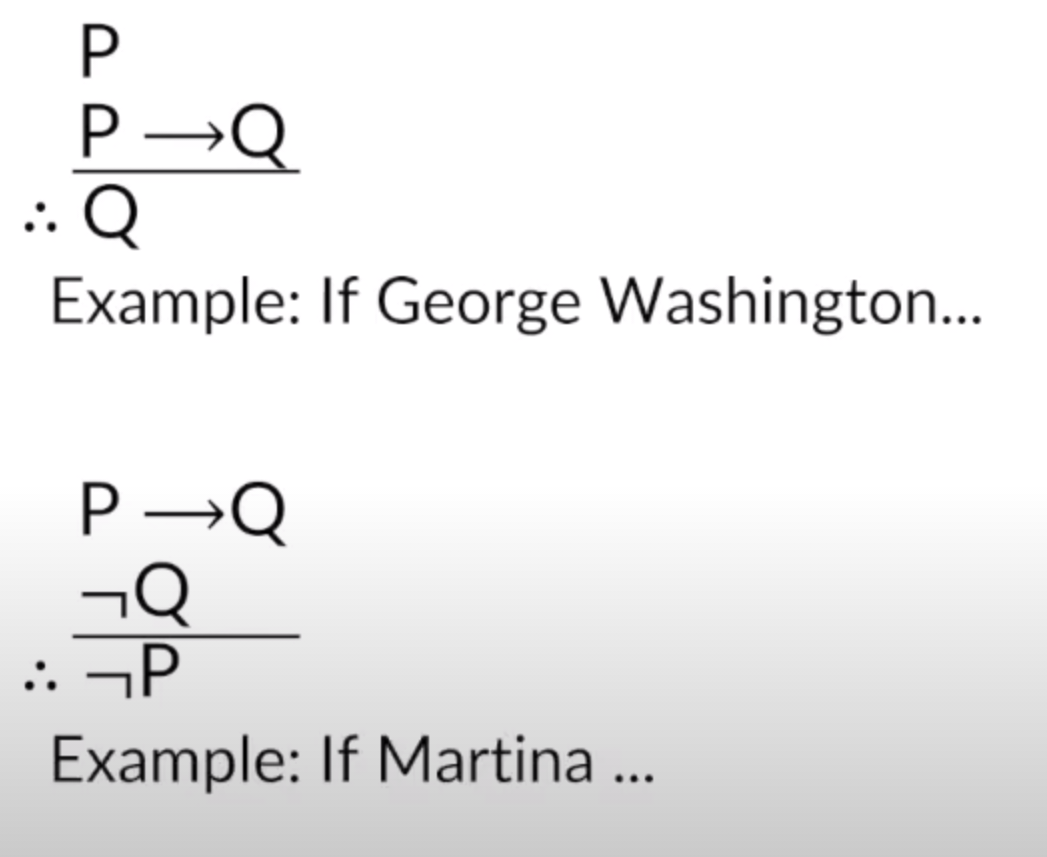
\includegraphics[width=8cm]{if1}
%	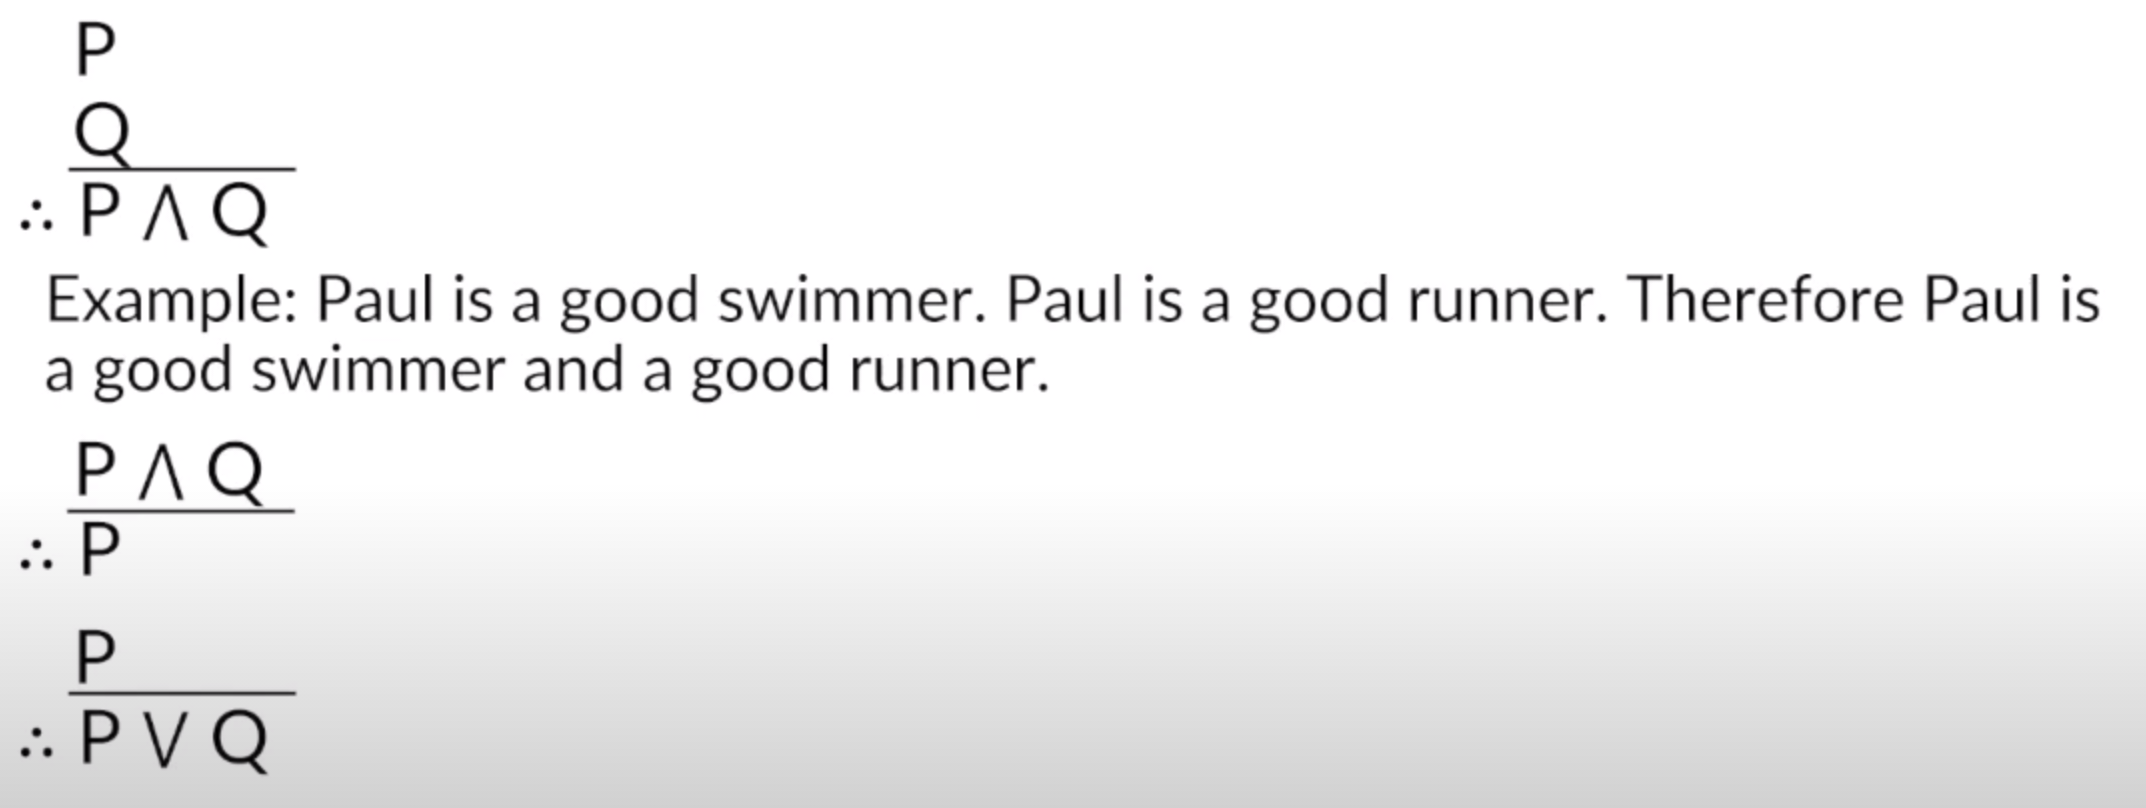
\includegraphics[width=16cm]{if2}
% \end{center}


% I wasted so much time making this lol
\bigbreak
\begin{center}
	\begin{tabular}{c c}
		\Longunderstack{
			$
			{
				\begin{array}{l}
					P \\
					P \implies Q \\
					\hline
					\therefore Q
				\end{array}
			}
			$ \\ \\
			{\tiny Ex: If George Washington...}
		} 
		& \Longunderstack{
			$
			{
				\begin{array}{l}
					P \implies Q \\
					\neg Q \\
					\hline
					\therefore \neg P
				\end{array}
			}
			$ \\ \\
			{\tiny Ex: If Martina...}
		} \\ \\ \\
		\Longunderstack{
			$
			{
				\begin{array}{l}
					P \land Q \\
					\hline
					\therefore P
				\end{array}
			}
			$
		} 
		& \Longunderstack{
			$
			{
				\begin{array}{l}
					P \\
					\hline
					\therefore P \lor Q
				\end{array}
			}
			$
		} \\ \\
		\multicolumn{2}{c}{
		\Longunderstack{
			$
			{
				\begin{array}{l}
					P \\
					Q \\
					\hline
					\therefore P \land Q
				\end{array}
			}
			$ \\ \\
			{\tiny Ex: Paul is a good swimmer. Paul is a good runner.} \\ {\tiny Therefore Paul is a good swimmer and a good runner}
		}}
	\end{tabular}
\end{center}

\intextnote[The items above the line can be combined/transformed into a new proof step defined below the line]

\pagebreak

\subsubsection*{Examples (finding conclusions)} 
\begin{enumerate}
	\item If the car was involved in the hit-and-run, then the paint would be chipped. But the paint is not chipped.
		\begin{itemize}[label={\faAngleRight}]
			\item "Car was involved in a hit-and-run" $\rightarrow P$
			\item "Paint would be chipped" $\rightarrow Q$
			\item "The paint is not chipped" $\rightarrow \neg Q$
			\item Conclusion: The car was not involved in a hit-and-run. From the second rule!
		\end{itemize}
	\item If the bill was sent today, then you will be paid tomorrow. You will be paid tomorrow.
		\begin{itemize}[label={\faAngleRight}]
			\item Nothing can be concluded from this. \smiley
		\end{itemize}
	\item If the program is efficient$_P$, it executes quickly$_Q$. Either the program is efficient$_P$, or it has a bug$_R$. However, the program does not execute quickly$_{\neg Q}$.
		\begin{itemize}[label={\faAngleRight}]
			\item "If the program is efficient" $\rightarrow P$
			\item "it executes quickly" $\rightarrow Q$
			\item "it has a bug" $\rightarrow R$
			\item "the program does not execute quickly" $\rightarrow \neg Q$
			\item We start by knowing $P \implies Q$ and $P \lor R$ and $\neg Q$...
			\item $(P \implies Q)$ and $\neg Q$ can imply $\neg P$
			\item We need to transform $P \lor R$ to use it: $P \lor R \equiv \neg (\neg P) \lor R \equiv \neg P \implies R$
			\item $\neg P \implies R$ and $\neg P$ (the first implication we isolated) now implies $R$ by the first inference rule.
		\end{itemize}
\end{enumerate}

\pagebreak

\subsubsection{Proving a Valid Argument}
Assuming the premises are true, apply a sequence of premises and derivation rules, which include the equivalence laws and inference.
\bigbreak
\textbf{General Steps} \\

\begin{enumerate}
	\item Identify all the premises (might need some transformations).
	\item \sidenote[Start with the RHS of the argument on the bottom of the list and work your way up] Think backwards. Start from what you want and then seek supporting premises, current results, and necessary equivalence laws and inference rules, until you reach the given premises.
	\item Write the proof sequence, where {\color{red}each step is either one premise or derived from previous step(s) using equivalence laws or inference rules.}
	
\end{enumerate}

\bigbreak

\subsubsection*{Examples}

\exheader[1]
Prove $(A \implies B) \land (\neg C \lor A) \land C \implies B$
\intextnote[This one is already in its standard form - so we just need to identify each part of the standard $P_1 \land P_2 \land P_3 ... \land P_n \implies Q$ form. At the end of this we want to prove that B is true.]

\begin{tabular}{r  l  l  l  l  l}
	$(A \implies B)$ & $\land$ & \Longunderstack{$(\neg C \lor A)$ \\ \tiny Implication Law} & $\land$ & $C$ & $\implies B$ \\
	$\downarrow$ & $\land$ & \Longunderstack{$C \implies A$ \\ \tiny first inference rule law} & $\land$ & $C$ & $\downarrow$ \\
	$(A \implies B)$ & $\land$ & \multicolumn{3}{l}{\Longunderstack{$A$ \\ \tiny also by first inf rule}} & $\downarrow$ \\
	\multicolumn{5}{c}{$B$} & $\implies B$
\end{tabular}

\intextnote[This is not usually how you would format these proofs, this table was to give you an idea of the actual process. The actual proof would look like the following;
\begin{enumerate}
	\item $A \implies B$
	\item $\neg C \lor A$
	\item $C$ 
	\item $C \implies A$ \hspace*{2cm} (2, Implication)
	\item $A$ \hspace*{3.3cm} (3,4)
	\item $B$ \hspace*{3.2cm} (1,5)
\end{enumerate}
You need to put every step in a seperate (numbered) line, starting with each component of the argument and then the transformations you do with the reason given. You dont need to name the law used but you need to mention the steps you combined to acheive the next part.]

\pagebreak

\exheader[2]
Prove $A \land (B \implies C) \land ((A \land B) \implies (D \lor \neg C)) \land B \implies D$
\intextnote[For this one focus on step 3 ($D \lor \neg C$) as your point to figure out this argument since its the only portion that has D in it.]
\begin{enumerate}
	\item $A$
	\item $B \implies C$
	\item $(A \land B) \implies (D \lor \neg C)$
	\item $B$
	\item $A \land B$ \hspace*{2.2cm} (1,4)
	\item $D \lor \neg C$ \hspace*{1.9cm} (3,5)
	\item $C \implies D$ \hspace*{1.5cm} (6, Commutative, Implication) - {\tiny Communicative used to swap C, D}
	\item $C$ \hspace*{3cm} (2,4)
	\item $D$ \hspace*{3cm} (7,8)
\end{enumerate}

\bigbreak

\exheader[3] Prove $(A \implies B) \land (\neg C \lor A) \land C \implies A \land B$
\intextnote[For this one notice that the right-hand side isn't a single letter anymore. We now need to focus on proving the whole $A\land B$ statement. So this problem is actually solved a bit backwards, start by writing the last steps ($A, B, A\land B$) and then go up and figure out how you can prove A.]
\begin{tabular}{c l l}
	1. & $A \implies B$ & \\
	2. & $\neg C \lor A$ & \\
	3. & $C$ & \\
	4. & $C \implies A$ & (2, Implication) \\
	5. & $A$ & (3,4) \\
	6. & $B$ & (1,5) \\
	7. & $A \land B$ & (5,6)
\end{tabular}

\intextnote[If instead this problem was looking for $A \lor B$, you could just prove either A or B to make the entire statement valid.]

\pagebreak


\subsubsection{The Deduction Method}

Now, what if the conclusion is in implication form? \\
There are two ways of solving for this form, the main one being \textbf{The Deduction Method...} \\

Suppose the argument has the form:
\begin{center}
	$ P_1 \land P_2 \land P_3 ... \land P_n \implies (R \implies S) $
\end{center}
where the conclusion itself is an implication. \cul{We can add R as an additional premise and then imply S}. In other words, we can have the argument:
\begin{center}
	$ P_1 \land P_2 \land P_3 ... \land P_n \land R \implies S $
\end{center}

\bigbreak \bigbreak

\subsubsection*{Examples}

\exheader[1] Prove $(A \implies B) \land (B  \implies C) \implies (A \implies C)$
\intextnote[Start with C at the bottom. Now the only way to validate C is if B is true, so make B step 4 and find the proper relations to make B true.]
Deduction: $(A \implies B) \land (B \implies C) \land A \implies C$ \\
\begin{tabular}{c l l}
	1. & $A \implies B$ & \\
	2. & $B \implies C$ & \\
	3. & $A$ & \\
	4. & $B$ & (1,3) \\
	5. & $C$ & (2,4) \\
\end{tabular}

\bigbreak

\exheader[2] Prove $\neg (A \land \neg B) \land (B \implies C) \implies (A \implies C)$ \\
Deduction: $\neg (A \land \neg B) \land (B \implies C) \land A \implies C$ \\
\begin{tabular}{c l l}
	1. & $\neg (A \land \neg B) $ & \\
	2. & $ B \implies C $ & \\
	3. & $A$ & \\
	4. & $\neg A \lor B $ & (1, DeMorgan's) \\
	5. & $A \implies B$ & (4, Implication) \\
	6. & $B$ & (3,5) \\
	7. & $C$ & (2,6)
\end{tabular}

%todo: excersise slide

\pagebreak

\subsection{Predicate Logic}



\define[A \textbf{predicate} represents the properties of/relations among objects. \\
Examples: \\
\hspace*{0.5cm}n \emph{is a perfect square} \\
\hspace*{0.5cm}x \emph{is greater than} y]

\subsubsection*{Often propositional logic is not enough!} 
There are several cases where propositional logic won't help us reach needed conclusions or information; \\
\begin{itemize}[label={}, leftmargin=*]
	\item Suppose we know that "All CS students must take CSCI 358". We cannot conclude that "Alice must take CSCI 358 where Alice is a CS student" using our current propositional logic knowledge.
	\item Statements that hold many objects must be enumerated;
	\begin{itemize}
		\item Example:
		\begin{itemize}
			\item If Alice is a CS student, then Alice must take CSCI358.
			\item If Bob is a CS student, then Bob must take CSCI358.
			\item If Chris is a CS student, then Chris must take CSCI358.
			\item ...
		\end{itemize}
		\item Solution: make statements with variables
		\begin{itemize}
			\item If x is a CS student, then x must take CSCI358.
		\end{itemize}
	\end{itemize}
	\item Statements that define the property of a group of objects;
	\begin{itemize}
		\item Example:
		\begin{itemize}
			\item All new cars must be registered.
			\item Some of the new CS students graduate with honor.
		\end{itemize}
		\item Solution: Make statements with quantifiers:
		\begin{itemize}
			\item Universal Quantifier - the property is satisfied by all members of the group.
			\item Existential Quantifier - at least one member of the group satisfies the property.
		\end{itemize}
	\end{itemize}
\end{itemize}

\pagebreak

\subsubsection{Predicate representation}
Predicates are represented like functions in other branches of maths; \\
\sidenote[Once we plug in a value for x, the predicate becomes a proposition]e.g $P(x)$ represents some predicate such as "x is a perfect square". \smallbreak
Note that predicates can involve multiple variables, e.g Q(x,y) is "x is greater than y." \bigbreak

The two main quantifiers are represented with $\forall$ and $\exists$ \\
\begin{itemize}
	\item Universal Quantifier: $\forall$
	\begin{itemize}
		\item Read as “for all,” “for every,” “for each,” or “for any.”
		\item Ex: $\forall x, x>0$ is read as “for any number $x$, $x$ is greater than 0.”
	\end{itemize}
	\item Existential Quantifier: $\exists$
	\begin{itemize}
		\item Read as “there exists one,” “there is,” “for at least one,” or “for some.”
		\item Example: $\exists x, x>0$ is read as “there exists a number x such that x is greater than zero.”
	\end{itemize}
\end{itemize}
\intextnote[\textnormal{When $\forall x P(x)$ or $\exists x P(x)$ is used, the domain must be specified.}]
\bigbreak

\subsubsection*{Truth Values of Predicates}
\smallbreak
\fontsize{9}{10}\selectfont
\begin{tabular}{|p{0.6in} | p{1.3in} | p{1.3in} | p{2.1in} |}
	\hline
	\rowcolor{lightgray} Predicate & True When... & False When... & Examples \\
	\hline \\
	$\forall x P(x)$ & If P(x) is true for \textbf{every} x in the domain & If there is \textbf{any} x in the domain such that P(x) is false & \Longunderstack[l]{$P(x)$ is $x+1>x$, $\forall P(x)$ is true \\ for the domain consisting of all \\ real numbers. \\ ----------------------------------------------- \\ $Q(x)$ is $x <2$. $\forall x Q(x)$ is false \\ for the domain consisting of all real \\ numbers because $Q(3)$ is false. \\ $x=3$ is a counterexample of $\forall x Q(x)$} \\ \\
	\hline \\
	$\exists x P(x)$ & There's is an x \textbf{anywhere} such that P(x) is true. & P(x) is false for \textbf{every} x & \Longunderstack[l]{$P(x)$ is $x > 3$. $\exists x P(x)$ is true \\ for the domain consisting of all real \\ numbers. Because when x=4, P(4) \\ is true.  \\ ----------------------------------------------- \\ $Q(x)$ is $X=x+1$. $exists x Q(x)$ is \\ false for the domain consisting of \\ all real numbers. Because $Q(x)$ is \\ false for every real number x} \\ \\
	\hline
	
\end{tabular}

\normalsize
\bigbreak

The quantifiers $\forall$ and $\exists$ have higher precedence than all logical connectives from propositional logic.

For Example: \\
\hspace*{1cm} $\forall x  P(x) \land Q(x)$ means $(\forall x  P(x)) \land Q(x)$ rather than $\forall x  (P(x) \land Q(x))$

\pagebreak

\subsubsection*{Negating Quantified Expressions}
\bigbreak
\bigbreak
\Large $\neg \forall x P(x) \equiv \exists x \neg P(x)$ 
\normalsize
\begin{itemize}[leftmargin=*, label={}]
	\item Example:
	\begin{itemize}
		\item Every CS Student Must take CSCI385.
		\item Negation: There is a CS student who doesn't have to take CSCI358
	\end{itemize}
\end{itemize}

\bigbreak
\bigbreak

\Large $\neg \exists x P(x) \equiv \forall x \neg P(x)$
\normalsize
\begin{itemize}[leftmargin=*, label={}]
	\item Example:
	\begin{itemize}
		\item There is s student in this class who has taken CSCI 262.
		\item Negation: Every student in this class has \textbf{not} taken CS262
	\end{itemize}
\end{itemize}


% 6:45 of the original video for the explination of why the implcation-based expression is wrong.
% for the russian examples bold the Every/ There is keywords because those denote whuch quanitifer u shuould use!

% loves everybody expression can be reiunterpreted as;
% there exists a person (x) for any person (y) where x loves y

\pagebreak

\subsubsection{Translating to Logical Expressions}
\subsubsection*{\small \emph{Converting statements to expressions}}

\bigbreak
\bigbreak

\subsubsection*{English to Logical Expressions}
\bigbreak

\exheader[1] Every parrot is beautiful
\begin{itemize}[leftmargin=*, label={}]
	\item Translation:
	\begin{itemize}
		\item Assume that the domain consists of all parrots.
		\begin{itemize}
			\item Let $B(x)$ denote "x is beautiful"
			\item Then $\forall x \ B(x)$
		\end{itemize}
		\item Assume that the domain consists of all animals.
		\begin{itemize}
			\item Let $P(x)$ denote "x is a parrot".
			\item Let $B(x)$ denote "x is beautiful"
			\item \sidenote[{\\ \fontsize{5}{12} \selectfont $\forall x (P(x) \land B(x))$ would be incorrect}]Then $\forall x \ (P(x) \implies B(x))$
		\end{itemize}
	\end{itemize}
\end{itemize}

\bigbreak

\exheader[2] There exists a beautiful parrot
\begin{itemize}[leftmargin=*, label={}]
	\item Translation:
	\begin{itemize}
		\item Assume that the domain consists of all parrots.
		\begin{itemize}
			\item Let $B(x)$ denote "x is beautiful
			\item Then $\exists x \ B(x)$
		\end{itemize}
		\item Assume that the domain consists of all animals.
		\begin{itemize}
			\item Let $P(x)$ denote "x is a parrot"
			\item Let $B(x)$ denote "x is beautiful"
			\item Then $\exists x \ (P(x) \land B(x))$
		\end{itemize}
	\end{itemize}
\end{itemize}\intextnote[$\exists x \ (P(x) \implies B(x))$ is an incorrect solution. If x is not a parrot then P(x) is false, since P(x) is attached to the start of the implication it would make the entire expression true (when it should be false)]

\pagebreak

\exheader[3] Let $P(x)$ denote "x speaks Russian" \\
\exheader[\indent] and let $Q(x)$ denote "x knows the computer language C++" \\
\exheader[\indent] Let the domain consist of all students at Mines. \\
\exheader[\indent] Translate the following into logical expressions;
\begin{itemize}[leftmargin=*, label={}]
	\item There is a student at Mines who speaks Russian and knows C++
	\begin{itemize}
		\item $\exists x \ (P(x) \land Q(x))$
	\end{itemize}
	\item There is a student at Mines who speaks Russian but doesn't know C++
	\begin{itemize}
		\item $\exists \ (P(x) \land \neg Q(x))$
	\end{itemize}
	\item Every student at Mines either speaks Russian or knows C++
	\begin{itemize}
		\item $\forall x \ (P(x) \lor Q(x))$
	\end{itemize}
	\item No student as Mines speaks Russian or knows C++
	\begin{itemize}
		\item $\forall x \ (\neg P(x) \land \neg Q(x))$
		\item or $\neg \exists x \ (P(x) \lor Q(x))$
	\end{itemize}
\end{itemize}

% todo add lions excercise if u need it!
\bigbreak
\horizline
\subsubsection*{Nested quantifiers}
\emph{More than one quantifier may be needed to represent the meaning of a statemente in predicate logic.}

\exheader[1] Every real number has its corresponding negative
\begin{itemize}[leftmargin=0.5cm, label={}]
	\item Assume that the domain consists of all real numbers
	\item Let $P(x,y)$ denote "$x + y = 0$"
	\item Then we can write $\forall x \ \exists y \ P(x,y)$
\end{itemize}

\bigbreak

\exheader[2] There is a person who loves everybody.
\begin{itemize}[leftmargin=0.5cm, label={}]
	\item Assume that the domain consists of all people
	\item Let $L(x,y)$ denote "$x$ loves $y$".
	\item Then we can write $\exists x \ \forall y \ L(x,y)$
\end{itemize}

\pagebreak


\subsubsection*{Order of quantifiers}
\bigbreak
When quantifiers are of the \textbf{same} type, the order \cul{doesn't} matter. \smallbreak
Example:
\begin{itemize}[leftmargin=0.8cm, label={\faAngleRight}]
	\item Assume that the domain consists of all real numbers.
	\item Let $P(x,y)$ denote "$x+y=y+x"$
	\item $\forall x \ \forall y \ P(x,y)$  represents “For every real number x, for every real number y, x + y = y + x.”
	\item $\forall y \ \forall x \ P(x,y)$  represents “For every real number y, for every real number x, x + y = y + x.”
	\item $\forall x \ \forall y \ P(x,y)$ and $\forall y \ \forall x \ P(x,y)$ have the same meaning!
\end{itemize}

\bigbreak
\bigbreak

When quantifiers are of \textbf{different} types, the order \cul{does} matter! \smallbreak
Example:
\begin{itemize}[leftmargin=0.8cm, label={\faAngleRight}]
	\item Assume that the domain consists of all real numbers.
	\item Let $Q(x,y)$ denote "$x + y = 0$"
	\item $\forall x \ \exists y \ Q(x,y)$  represents “For every real number x, there is a real number y, such that x + y = 0.”
	\item $\exists y \ forall x \ Q(x,y)$ represents “There is a real number y, such that for every real number x, x + y = 0.”
	\item $\forall x \ \exists y \ Q(x,y)$ and $\exists y \ forall x \ Q(x,y)$ have different meanings!
\end{itemize}

\bigbreak
\bigbreak

Ex: Let $Q(x,y,z)$ be "$x+y=z"$ and assume that the domain consists of all real numbers. \\
\begin{center}
	$\forall x \ \forall y \ \exists z \ Q(x,y,z) \not\equiv \exists z \ \forall x \ \forall y \ Q(x,y,z)$
\end{center}

\pagebreak

\vspace*{-2cm} \subsubsection{Translation Examples}
\subsubsection*{English to Logical Expression Examples}
\bigbreak

\exheader[1] Given the two unique statements;
\begin{enumerate}
	\item John loves only Mary (If John loves any person, then that person is Mary.)
	\item Only John loves Mary (If any person loves Mary, then that person is John.)
\end{enumerate}
Let $J(x)$ be "x is John". let M(x) be "x is Mary". Let L(x,y) be "x loves y". The domain consists of all people.
\begin{enumerate}
	\item John loves only Mary.
	\begin{itemize}[leftmargin=0.3cm, label={\faAngleRight}]
		\item For any person x, if x is John, then if it loves any person y, then y is Mary.
		\item $\forall x \ (J(x) \implies \forall y (L(x,y) \implies M(y)))$ \\ Or $\forall x \ \forall y \ (J(x) \land L(x,y) \implies M(y))$
	\end{itemize}
	\item Only John loves Mary.
	\begin{itemize}[leftmargin=0.3cm, label={\faAngleRight}]
		\item For any person x, if x is Mary, then if any person y loves x, then y is John.
		\item $\forall x \ (M(x) \implies \forall (L(y,x) \implies J(y)))$ \\ Or $\forall x \ \forall y \ (M(x) \land L(y,x) \implies J(y))$
	\end{itemize}
\end{enumerate}
\bigbreak
\exheader[2] Given that; D(x) is "x is a dog". R(x) is "x is a rabbit". C(x,y) is "x chases y". The domain consists of all animals. \\ Translate the following;
\begin{enumerate}
	\item All dogs chase rabbits.
	\begin{itemize}[leftmargin=0.3cm, label={\faAngleRight}]
		\item For any animal, if it is a dog, then for any other animal, if that animal is a rabbit, then the dog chases it.
		\item $\forall x \ (D(x) \implies \forall y (R(y) \implies C(x,y)))$
	\end{itemize}
	\item Some dogs chase all rabbits.
	\begin{itemize}[leftmargin=0.3cm, label={\faAngleRight}]
		\item There is some animal that is a dog and, for any other thing, if that animal is a rabbit, then the dog chases it.
		\item $\exists x \ \forall y (D(x) \land (R(y) \implies C(x,y)))$
	\end{itemize}
	\item Only dogs chase rabbits.
	\begin{itemize}[leftmargin=0.3cm, label={\faAngleRight}]
		\item For any animals, if it is a rabbit then, if any animal chases it, that animal is a dog.
		\item $\forall y \ (R(y) \implies \forall x (C(x,y) \implies D(x)))$
		\item or: For any two animals, if one is a rabbit and the other chases it, then the other is a dog.
		\item $\forall y \ \forall x \ (R(y) \land C(x,y) \implies D(x))$
	\end{itemize}
\end{enumerate}
\pagebreak
\subsubsection*{Mathematical Statements to Logical Expression Examples}
\bigbreak

\exheader[1] Translate "The sum of two positive integers is always positive." 
\begin{itemize}[leftmargin=*, label={}]
	\item Assume that the domain consists of all integers.
	\begin{itemize}
		\item For every two integers, if they are both positive, then the sum of them is positive.
		\item $\forall x \ \forall y \ (x > 0 \land y > 0 \implies (x + y > 0))$
	\end{itemize}
	\item Assume that the domain consists of all positive integers.
	\begin{itemize}
		\item For every two positive integers, the sum of them is positive.
		\item $\forall x \ \forall y \ (x+y>0)$
	\end{itemize}
\end{itemize}

\exheader[2] Translate "The difference of two positive integers is not necessarily positive."
\begin{itemize}[leftmargin=*, label={}]
	\item Assume that the domain consists of all integers.
	\begin{itemize}
		\item It is not the case that, for every two integers, if they are both positive, then the difference of them is positive.
		\item $\neg \forall x \ \forall y \ (x > 0 \land y > 0 \implies (x - y > 0))$ \\ Or: $\exists x \ \exists y ((x > 0 \land y > 0) \land (x-y \le 0))$
	\end{itemize}
\end{itemize}

\bigbreak
\horizline

\subsubsection*{Logical Expressions to English Examples}
\bigbreak
\exheader[1] Translate: $\forall x (C(x) \lor \exists y (C(y) \land F(x,y)))$, where $C(x)$ denotes "x has a computer," $F(x,y)$ denotes "x and y are friends," and the domain consists of all Mines students.
\begin{itemize}[leftmargin=0.3cm, label={}]
	\item For every student x at Mines, x has a computer or there is a student y such that y has a computer and x and y are friends.
	\item Simplifies to: Every student at Mines has a computer or a friend that has a computer.
\end{itemize}

\exheader[2] Translate: $\exists x \ \forall y \ \forall z ((F(x,y) \land F(x,z) \land (y \ne z)) \implies \neg F(y,z))$, where $F(x,y)$ denotes "x and y are friends," and the domain consists of all students at Mines.
\begin{itemize}[leftmargin=0.3cm, label={}]
	\item $\exists x \ \forall y \ \forall z ((F(x,y) \land F(x,z) \land (y \ne z)) \implies \neg F(y,z))$ means that if students x and y are friends, and students x and z are friends, and y and z are not the same student, then y and z are not friends.
	\item There is a student x such that for every student y and every student z other than y, if x and y are friends, x and z are friends, then y and z are not friends.
	\item There is a Mines student none of whose friends are friends.
\end{itemize}

\pagebreak

\subsubsection{Negating Nested Quantifiers}
\bigbreak
\textbf{General Principle}: Moving a $\neg$ across a quantifier changes the kind of quantifier.
\bigbreak
What is the negation of $\forall x \ \exists y (xy = 1)?$
\begin{itemize}[label={}]
	\item Let $P(x)$ denote $\exists y (xy = 1)$
	\item Then we know how to negate $\forall x \ P(x)$
	\item $\neg \forall x \ P(x) \equiv \exists x \ \neg P(x)$
	\item In addition, $\neg P(x) \equiv \neg \exists y \ (xy = 1) \equiv \forall y \ (xy \ne 1)$
	\item Therefore, the negation of $\forall x \ \exists y \ (xy =1)$ is $\exists x \ \forall y (xy \ne 1)$
\end{itemize}

\pagebreak


\subsubsection{Arguments In Predicate Logic}
Just like propositional logic, we need to utilize inference rules to prove these arguments.

\bigbreak
\textbf{Basic examples}: (Assume the domain is all Mines CS students.)
\begin{enumerate}
	\item All the CS students must take CSCI 358. Thus some CS students must take CSCI 358.
	\begin{itemize}[label={\faAngleRight}]
		\item $\forall x \ P(x) \implies \exists x \ P(x)$ \textcolor{green}{\checkmark}
		\item If every element has property P, then some element has property P
	\end{itemize}
	\item All the CS students must take CSCI 358. Thus Alice must take CSCI 358, where Alice is a CS student
	\begin{itemize}[label={\faAngleRight}]
		\item \sidenote[The $P(a)$ here represents a "constant" Alice whom is a particular element within the domain] $\forall x \ P(x) \implies P(a)$, where $a$ is a constant \textcolor{green}{\checkmark}
		\item If every element has property P, then a particular element has property P.
	\end{itemize}
	\item All the CS students must take CSCI 261 and CSCI 358. Thus all the CS students must take CSCI 261 and all the CS students must take CSCI 358.
	\begin{itemize}[label={\faAngleRight}]
		\item $\forall x \ (P(x) \land Q(x)) \implies \forall x \ P(x) \land \forall x \ Q(x)$ \textcolor{green}{\checkmark}
		\item If both P and Q are true for all the elements, then P is true for all elements and Q is true for all elements (duh)
	\end{itemize}
	\item \sidenote[This one also just doesn't make intuitive sense. Try rewriting arguments like this into English and see if they make sense!]Some CS students graduate with honors. Thus all the CS students graduate with honors.
	\begin{itemize}[label={\faAngleRight}]
		\item $\exists x \ P(x) \implies \forall x \ P(x)$ \textcolor{red}{\faClose}
		\item If some element has property P, then all the elements have property P.
	\end{itemize}
\end{enumerate}


\pagebreak
\vspace*{-1.5cm}
\textbf{All the equivalence laws and inference rules still hold!} \\

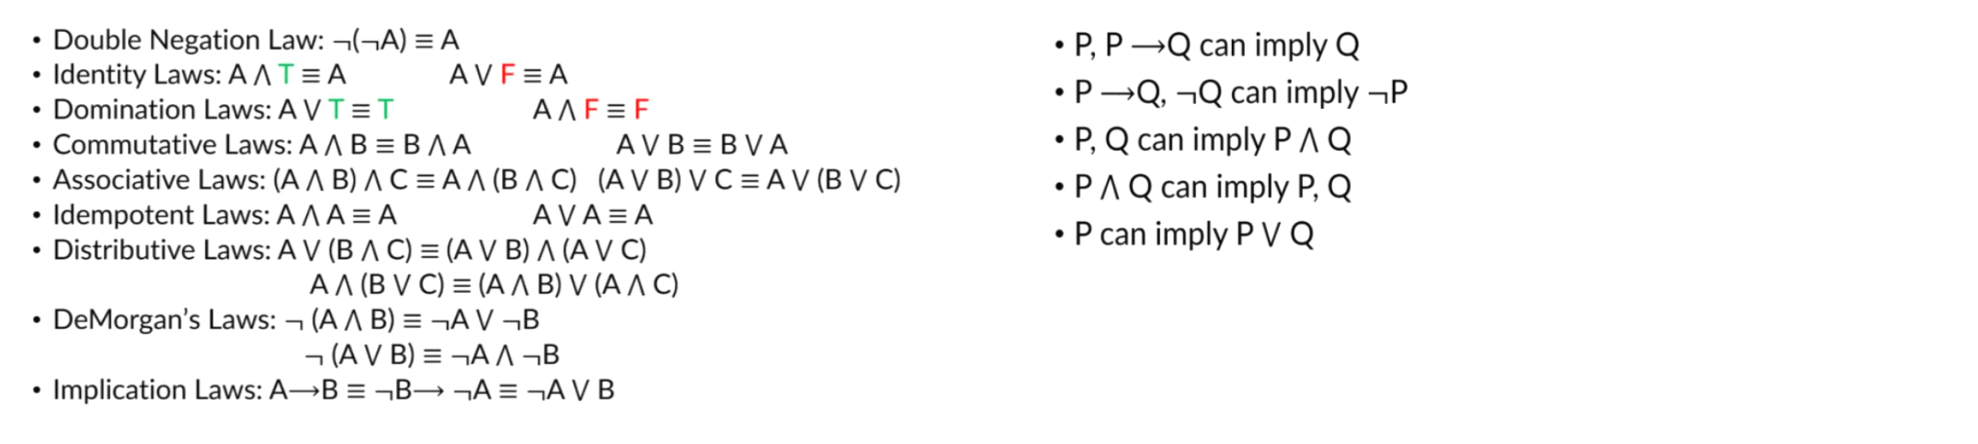
\includegraphics[width=\textwidth]{images/compiled rules.png}

However, these rules are not enough, predicates will utilize \cul{four new inference rules};
{\large
\begin{itemize}[label={}, leftmargin=0.3cm]
	\item \textcolor{blue}{\cul{Universal Instantiation}} \\ $\forall x \ P(x)$ can imply $P(c)$, where $c$ is a particular element or any arbitrary element in the domain.
	\begin{itemize}
		\item {\small If for any $x$ in which $P(x)$ is true, then $P(c)$ must also be true. More intuitively thought as the fact that if all elements in the domain have property "P", then any element (particular or arbitrary within the domain) must also have this property.}
	\end{itemize}
	\item \textcolor{blue}{\cul{Existential Instantiation}} \\ $\exists x \ P(x)$ can imply $P(a)$, where $a$ is a particular element \textcolor{red}{not previously used in a proof sequence}
	\begin{itemize}
		\item {\small $\exists x P(x)$ means there must be some element in the domain that has property "P". Even though we don't know \emph{exactly} what that element is, we can use the letter "$a$" to represent this particular element. }
	\end{itemize}
	\item \textcolor{blue}{\cul{Universal Generalization}} \\ $P(c)$ can imply $\forall x \ P(x)$, where $c$ is an arbitrary element in the domain.
	\begin{itemize}
		\item {\small If any/every arbitrary element in the domain has property P ($P(c)$ always true), we can obviously say $\forall x P(x)$}
	\end{itemize}
	\item \textcolor{blue}{\cul{Existential Generalization}} \\ $P(a)$ can imply $\exists x \ P(x)$, where $a$ is a particular element.
	\begin{itemize}
		\item {\small If a particular element in the domain has property "P", we can obviously say $\exists x \  P(x)$ }
	\end{itemize}
\end{itemize}
}
\bigbreak
\faInfoCircle \ \emph{The first two rules can be used to remove the quantifiers in front of the predicates. \\ The last two rules can be used to add quantifiers to the front of predicates}
\bigbreak
\textbf{Let's look at all of these in more depth...}


\pagebreak
\subsubsection*{Universal Instantiation (UI)}
$\forall x \ P(x)$ can imply $P(c)$, where $c$ is a particular element or any arbitrary element in the domain. 
\begin{itemize}[label={}, leftmargin=0.3cm]
	\item \textcolor{blue}{Restrictions:} If $c$ is a variable, it cannot be already in $P(x)$
	\item An \textcolor{red}{\textbf{incorrect}} use of UI would be saying \textcolor{red}{$\forall x \ \exists y \ P(x,y)$ implies $\exists y \ P(y,y)$}
	\begin{itemize}[label={}]
		\item For example, in the integer domain, if $P(x,y)$ means "$ y > x $" then $\forall x \ \exists y \ P(x,y)$ is true, but $\exists y \ P(y,y)$ is false (y can't be greater than y \faSmileO).
	\end{itemize}
	\item \cul{Example}
	\begin{itemize}[label={}]
		\item Prove the following argument is valid: "All CS students must take CSCI358. Alice is a CS student. Therefore Alice must take CSCI 358." The domain consists of all Mines students.
		\item Let $C(x)$ be "$x$ is a CS student." $s$ is a constant symbol. $D(x)$ is "$x$ has to take CSCI358"
		\item The argument would be: $\forall x (C(x) \implies D(x)) \land C(s) \implies D(s)$
		{\small \begin{enumerate}
			\item $\forall x \ (C(x) \implies D(x))$
			\item $C(s)$
			\item $C(s) \implies D(s)$ (1,UI)
			\item $D(s)$ \hspace*{1.75cm} (2,3)
		\end{enumerate}
		}
	\end{itemize}
\end{itemize}

\pagebreak

\subsubsection*{Existential Instantiation (EI)}
$\exists x \ P(x)$ can imply $P(a)$, where $a$ is a particular element \textcolor{red}{not previously used in a proof sequence}
\begin{itemize}[label={}, leftmargin=0.3cm]
	\item In English: If P is true for some element of the domain, we can give that element a specific notation.
	\item \textcolor{blue}{Restrictions:} $a$ must not be used before!
	\item Incorrect Uses of EI:
	\begin{itemize}
		\item \textcolor{red}{$\exists \ P(x,a)$ CANNOT imply $P(a,a)$} \\ For example: in the integer domain, let P$(x,y)$ denote $x > y$ and $a = 1$
		\item \textcolor{red}{$\forall x  \ \exists y \ Q(x,y)$ CANNOT imply $\forall x Q(x,a)$} \\ For example: in the integer domain, let $Q(x,y)$ denote that $x > y.$
	\end{itemize}
	\item \cul{Example}: $\forall x \ (P(x) \implies Q(x)) \land \exists y \ P(y) \implies Q(a)$
	\begin{center}
		\begin{tabular}{l l l}
			1. & $\forall x \ (P(x) \implies Q(x))$ & \\
			2. & $\exists y \ P(y)$ & \\
			3. & $P(a)$ & (2,EI) \\
			4. & $P(a) \implies Q(a)$ & (1,UI) \\
			5  & $Q(a)$ & (3,4)  
		\end{tabular}
	\end{center}
\end{itemize}
\todo[inline]{\tiny TODO: Update these incorrect use examples, what do these mean?}
% rewatch the video for the EI - he explains the right and wrong way to do it - make sure to put down both to better understand the restrictions of this method.


\pagebreak


\subsubsection*{Universal Generalization (UG)}
$P(c)$ can imply $\forall x \ P(x)$, where $c$ is an arbitrary element in the domain.
\begin{itemize}[label={}, leftmargin=0.3cm]
	\item In English: If $P(c)$ is true and c is arbitrary, then we can conclude $\forall x \ P(x)$
	\item No weird restrictions or common misuses.
	\item \cul{Example}: $\forall x \ (P(x) \implies Q(x)) \land \forall x \ P(x) \implies \forall x \ Q(x)$
	\begin{center}
		\begin{tabular}{l l l}
			1. & $\forall x \ (P(x) \implies Q(x))$ & \\
			2. & $\forall x \ P(x)$ & \\
			3. & $P(c) \implies Q(c)$ & (1,UI) \\
			4. & $P(c)$ & (2,UI) \\
			5. & $Q(c)$ & (3,4) \\
			6. & $\forall x \ Q(x)$ & (5,UG)
		\end{tabular}
	\end{center}
\end{itemize}

\pagebreak

\subsubsection*{Existential Generalization (EG)}
$P(a)$ can imply $\exists x \ P(x)$, where $a$ is a particular element.
\begin{itemize}[label={}, leftmargin=0.3cm]
	\item In English: Something has been named as having property P, so we can say that there exists something that has property P.
	\item \textcolor{blue}{Restrictions:} x must not appear in $P(a)$
	\item Incorrect Uses of EG:
	\begin{itemize}
		\item \textcolor{red}{$P(z,y)$ CANNOT imply $\exists y P(y,y)$} \\ For example: In the positive integer domain, let $P(x,y)$ mean that $y > x$, and $a$ stands for 0, then $y>0$ does not mean $y>y$
	\end{itemize}
	\item Example: $\forall x \ P(x) \implies \exists x \ P(x)$
	\begin{center}
		\begin{tabular}{l l l}
			1. & $\forall x \ P(x)$ & \\
			2. & $P(a)$  & (1,UI) \\
			3. $\exists x \ P(x)$ & (2,EG)
		\end{tabular}
	\end{center}
\end{itemize}

\pagebreak

\subsubsection*{Proving a Valid Predicate Logic Argument (examples)}
\horizline
\cul{General Steps:}
\begin{enumerate}[leftmargin=*]
	\item Strip off the quantifiers.
	\item Work with the separate statements.
	\item Insert quantifiers, as necessary.
\end{enumerate}
\horizline

\exheader[1] $\forall x \ (P(x) \land Q(x)) \implies \forall x \ P(x) \land \forall x \ Q(x)$ \\
\begin{tabular}{c l l}
	1. & $\forall x \ (P(x) \land Q(x))$ & \\
	2. & $P(c) \land Q(c)$ & (1,UI) \ \ {\tiny \faInfoCircle \ You can use the same arbitrary element c for both P and Q} \\
	3. & $P(c)$ & (2) \\
	4. & $Q(c)$ & (2) \\
	5. & $\forall x \ P(x) $ & (3,UG) \\
	6. & $\forall x \ Q(x) $ & (4,UG) \\
	7. & $\forall x \ P(x) \land \forall x \ Q(x)$ & (5,6)
\end{tabular}

\bigbreak \bigbreak

\exheader[2] {\small Prove the following argument is valid: “A student in this class has not attended any in-person classes. Everyone in this class passed the first exam. Therefore someone who passed the first exam has not attended any in-person classes.”
\\ Let C(x) be “x is in this class,” B(x) be “x has attended in-person classes,” and P(x) be “x passed the first exam.” Let the domain consist of all Mines students.}
\\ \sidenote[Its easier to figure this one out in reverse, follow the proof from the bottom up as a process of what we need preceeded by what we use to get it!] $\exists x \ (C(x) \land \neg B(x)) \land \forall x \ (C(x) \implies P(x)) \implies \exists x \ (P(x) \land \neg B(x))$ \\ \\
\begin{tabular}{c l l}
	1. & $\exists x \ (C(x) \land \neg B(x))$ & \\
	2. & $\forall x \ (C(x) \implies P(x))$ & \\
	3. & $C(a) \land \neg B(a)$ & (1,EI) \\
	4. & $C(a)$ & (3)\\
	5. & $C(a) \implies P(a)$ & (2, UI) \\
	6. & $P(a)$ & (4,5) \\
	7. & $\neg B(a)$ & (3) \\
	8. & $P(a) \land \neg B(a)$ & (6,7) \\
	9. & $\exists x (P(x) \land \neg B(x))$ & (8,EG)
\end{tabular}
\todo[inline]{TODO: Add HW answers as examples later, HW had some weird situations that would be good to note.}


\pagebreak
\subsection{Chapter 1 Cheatsheet}
\smallbreak
\begin{tabular}{|c|c|c|c|c|l}
	\hline
	\rowcolor{lightgray} \multicolumn{5}{|c|}{Connectives} \\
	\hline
	\hline
	$\land$ & $\lor$ & $\implies$ & $\iff$ & $\neg$ \\
	AND & OR & IMPLIES & BICONDITIONAL & NEGATION \\
	\hline
	A and B & A or B & If A then B & A if and only if B & Not A \\
	\hline
	Both True & Either's True & $\star$ & A = B & - \\
	\hline
\end{tabular} 
\begin{tabular}{l}
	\\
	\\
	\\
	\\
	\\
	{\tiny $\leftarrow$ true when} \\
	\\
\end{tabular}
\emph{$\star$ - An implication is only false when A is true and B is false. {\tiny ref truth tables (1.2.2)}}
\bigbreak

\small
\begin{tabular}{ |p{0.4\textwidth}|p{0.5\textwidth}|}
	\hline
	\rowcolor{lightgray} \multicolumn{2}{|c|}{Equivalence Laws} \\
	\hline
	\hline
	Double Negation Laws	& \begin{itemize}[leftmargin=*, label={}, noitemsep,topsep=0pt, parsep=0pt]
		\item $\neg(\neg A) \equiv A$
	\end{itemize} \\
	\hline
	Identity Laws	& \begin{itemize}[leftmargin=*, label={}, noitemsep,topsep=0pt]
		\item $A \land T \equiv A$
		\item $A \lor F \equiv A$
	\end{itemize} \\
	\hline
	Domination Laws	& \begin{itemize}[leftmargin=*, label={}, noitemsep,topsep=0pt]
		\item $A \lor T \equiv T$
		\item $A \land F \equiv F$
	\end{itemize} \\
	\hline
	Communicative Laws	& \begin{itemize}[leftmargin=*, label={}, noitemsep,topsep=0pt]
		\item $A \land B \equiv B \land A$
		\item $A \lor B \equiv B \lor A$
	\end{itemize} \\
	\hline
	Associative Laws	& \begin{itemize}[leftmargin=*, label={}, noitemsep,topsep=0pt]
		\item $(A \land B) \land C \equiv A \land (B \land C)$
		\item $(A \lor B) \lor C \equiv A \lor (B \lor C) $
	\end{itemize} \\
	\hline
	Idempotent Laws	& \begin{itemize}[leftmargin=*, label={}, noitemsep,topsep=0pt]
		\item $A \land A \equiv A$
		\item $A \lor A \equiv A$
	\end{itemize} \\
	\hline
	Distributive Laws	& \begin{itemize}[leftmargin=*, label={}, noitemsep,topsep=0pt]
		\item $A \lor (B \land C) \equiv (A \lor B) \land (A \lor C)$
		\item $A \land (B \lor C) \equiv (A \land B) \lor (A \land C)$
	\end{itemize} \\
	\hline
	DeMorgans Laws	& \begin{itemize}[leftmargin=*, label={}, noitemsep,topsep=0pt]
		\item $\neg (A \land B) \equiv \neg A \lor \neg B$
		\item $\neg (A \lor B) \equiv \neg A \land \neg B$
	\end{itemize} \\
	\hline
	Implication Laws	& \begin{itemize}[leftmargin=*, label={}, noitemsep,topsep=0pt]
		\item $A \implies B \equiv \neg B \implies \neg A$
		\item $A \implies B \equiv \neg A \lor B$
	\end{itemize} \\
	\hline
	Not a law, but helpful biconditional equivalence...	& \begin{itemize}[leftmargin=*, label={}, noitemsep,topsep=0pt]
		\item $A \iff B \equiv (A \implies B) \land (B \implies A)$
	\end{itemize} \\
\hline
\end{tabular}
\normalsize
\pagebreak

\begin{tabular}{|c|c|}
	\hline
	\rowcolor{lightgray} \multicolumn{2}{|c|}{Inference Rules} \\
	\hline
	\hline
	$
			{
				\begin{array}{l}
					P \\
					P \implies Q \\
					\hline
					\therefore Q
				\end{array}
			}
	$ & Modus Ponens \\
	\hline
	$
			{
				\begin{array}{l}
					P \implies Q \\
					\neg Q \\
					\hline
					\therefore \neg P
				\end{array}
			}
	$ & Modus Tollens \\
	\hline
	$
			{
				\begin{array}{l}
					P \implies Q \\
					Q \implies R \\
					\hline
					\therefore P \implies R
				\end{array}
			}
	$ & Hypothetical Syllogism \\
	\hline
	$
			{
				\begin{array}{l}
					P \lor Q \\
					\neg P \\
					\hline
					\therefore Q
				\end{array}
			}
	$ & Disjunctive Syllogism \\
	\hline
	$
			{
				\begin{array}{l}
					P \\
					Q \\
					\hline
					\therefore P \land Q
				\end{array}
			}
	$ & Conjunction \\
	\hline
	$
			{
				\begin{array}{l}
					P \lor Q \\
					\neg P \lor R \\
					\hline
					\therefore Q \lor R
				\end{array}
			}
	$ & Resolution \\
	\hline
	$
			{
				\begin{array}{l}
					P \\
					\hline
					\therefore P \lor Q
				\end{array}
			}
	$ & Addition \\
	\hline
	$
	{
		\begin{array}{l}
			P \land Q \\
			\hline
			\therefore P
		\end{array}
	}
$ & Simplification \vspace*{-0.5cm} \\
&   {\tiny \faInfoCircle you're basically "pulling" p out to its own line} \\
\hline
\end{tabular}

\begin{tabular}{|c|c|}
	\hline
	\rowcolor{lightgray} \multicolumn{2}{|c|}{Quantified Inference Rules} \\
	\hline
	\hline
\end{tabular}



\smallbreak
\emph{\faInfoCircle These names don't really matter for this class}

\todo[inline]{TODO: Quantified Statement Inf Rules (ref saved screenshot) + other misc helpful stuff like negations of quantifiers. Just look up and copy-paste important details $\smiley$}





\pagebreak

\section{Proofs}
\bigbreak
\bigbreak
\subsection{Proof Basics}
\bigbreak
\textbf{Some New Terminology}
\begin{itemize}[leftmargin=0.5cm, label={\faAngleRight}]
	\item A \textbf{theorem} is a proposition that can be shown to be true.
	\item A \textbf{lemma} is a preliminary proposition useful for proving later propositions.
	\item A \textbf{corollary} is a proposition that can be established directly from a theorem.
	\item A \textbf{conjecture} is a proposition that is being proposed to be a true statement.
	\item Propositions that are simply accepted as true are called \textbf{axioms.}
	\begin{itemize}[label={\tiny ex:}]
		\item For all real numbers x and y, x + y = y + x 
		\item There is a straight-line segment between every pair of points.
	\end{itemize}
	\item A \textbf{proof} is a valid argument that establishes the truth of a statement.
	\begin{itemize}[leftmargin=*, label={}]
		\item \vspace*{-0.5cm} {\tiny Can use axioms, premises (if any) and previously proved theorems.}
	\end{itemize}
\end{itemize}

\subsubsection*{Common Theorem Forms}
\begin{itemize}[leftmargin=*, label={}]
	\item T
	\begin{itemize}[label={\tiny ex:}, leftmargin=1.25cm]
		\item "$\sqrt{2}$ is not a rational number."
	\end{itemize}
	\item \textbf{$\exists x T(x)$}
	\begin{itemize}[label={\tiny ex:},  leftmargin=1.25cm]
		\item "There exists one integer $n$ such that $n^2 + n + 41$ is composite"
		\begin{itemize}
			\item {\small You would have to find an element $a$ in the domain such that $T(a)$ is true and then apply Existential Generalization}
			\item {\small To disprove, prove that T(x) is false for all elements in the domain}
		\end{itemize}
	\end{itemize}
	\item $\forall x \ (P(x) \implies Q(x))$
	\begin{itemize}[label={\tiny ex:}, leftmargin=1.25cm]
		\item "For every integer n, if $3n+2$ is odd, then $n$ is odd."
		\begin{itemize}
			\item {\small You would have to show that $P(c) \implies Q(c)$, where $c$ is an arbitrary element of the domain, and then apply Universal Generalization}
			\item {\small Show that Q is true if P is true.}
			\item {\small To disprove, find a element $e$ such that $P(e)$ is true, but $Q(e)$ is false.}
		\end{itemize}
	\end{itemize}
	\item $\forall x \ (P \iff Q)$
	\begin{itemize}[label={\small \faInfoCircle}, leftmargin=1.25cm]
		\item Proving $(P \iff Q)$ is equivalent to proving $(P \implies Q) \land (Q \implies P)$
	\end{itemize}
\end{itemize}
\pagebreak

\subsection{Proof Methods}
There are four main proof methods; \\
{\small
\begin{tabular}{c c c c}
	Direct Proof & Proof by Contraposition & Proof by Contradiction & Proof by Cases
\end{tabular}
}	 

\horizline

\subsubsection{Direct Proof}
Directly show that if P is true, then Q must be true, using
axioms, definitions, and previously proven theorems, together
with inference rules. 
\bigbreak
\textbf{Examples} \\
\exheader[1] Prove that "If $n$ is odd, then $n^2$ is odd." \\ Proof:
\vspace*{-0.25cm}
\begin{itemize}[leftmargin=*, label={}]
	\item Assume that $n$ is odd, then $n = 2k +1$, where k is some integer.
	\item \sidenote[n is odd when $n = 2(...) + 1$. We have to figure out how to transform $n^2$ into this form.] We have $n^2 = (2k+1)^2 = 4k^2 + 4k + 1 = 2(2k^2 + 2k) +1$.
	\item Therefore, $n^2$ is an odd integer.
\end{itemize}

\bigbreak

\exheader[2] Prove that "If $m$ and $n$ are both perfect squares, then $mn$ is also a perfect square.” \\ Proof:
\vspace*{-0.25cm}
\begin{itemize}[label={}, leftmargin=*]
	\item Assume that $m$ and $n$ are both perfect squares, then $m = s^2$ and $n = t^2$, where $s$ and $t$ are some integers.
	\item We have $mn = s^2 t^2 = (st)^2 $
	\item Therefore, $mn$ is a perfect square.
\end{itemize}

\pagebreak

\subsubsection{Proof by Contraposition}
Instead of proving $P \implies Q$, prove $\neg Q \implies \neg P$. \\
We do this because we can then utilize the implication law: 
\begin{center}
	$P \implies Q \equiv \neg Q \implies \neg Q$
\end{center}
\bigbreak
\textbf{Examples} \\
\exheader[1] Prove that "For any integer $n$, if $n^2$ is even, then $n$ is even." \\ Proof:
\vspace*{-0.25cm}
\begin{itemize}[leftmargin=*, label={}]
	\item Contraposition: "If $n$ is odd, then $n^2$ is odd."
	\item (Reference example 1 of the direct proof)
	\item We have now proven this theorem.
\end{itemize}

\bigbreak

\exheader[2] Prove that "If $3n + 2$ is odd for an integer n, then n is odd." \\ Proof:
\vspace*{-0.25cm}
\begin{itemize}[leftmargin=*, label={}]
	\item Contraposition: "If n is even, then 3n + 2 is even"
	\item Assume that n is even, then $n = 2k$, where k is some integer.
	\item We have $3n + 2 = 6k + 2 = 2(3k+1)$
	\item Therefore $3n + 2$ is even.
	\item We have proved the theorem "If $3n + 2$ is odd then $n$ is odd."
\end{itemize}

\bigbreak

\exheader[3] Prove that "If $r$ is irrational, then $\sqrt{r}$ is also irrational" \\ Proof:
\vspace*{-0.25cm}
\begin{itemize}[leftmargin=*, label={}]
	\item Contraposition: "if $\sqrt{r}$ is rational, then r is rational."
	\item Assume that $\sqrt{r}$ is rational.
	\item There exists integers $p$ and $q$ (no common factors), such that $\sqrt{r} = \frac{p}{q}$
	\item Squaring both sides gives $r = \frac{p^2}{q^2}$
	\item Since $p^2$ and $q^2$ are integers, $r$ is also rational.
	\item This proves the theorem.
\end{itemize}

\pagebreak

\subsubsection{Proof by Contradiction}
Assume we want to prove $S$ is true. \\ Now, suppose we can find a contradiction $C$ such that $\neg S \implies C$ is true. \\ Since $C$ is false, but $\neg S \implies C$ is true, then S must be true.
\bigbreak
\textbf{Examples} \\
\exheader[1] Prove that '$\sqrt{2}$ is not a rational number." \\ Proof:
\vspace*{-0.25cm}
\begin{itemize}[leftmargin=*, label={}]
	\item Assume that $\sqrt{2}$ is a rational number.
	\item Then $\sqrt{2} = \frac{p}{q}$ where $p$ and $q$ have no common factors and $2 = \frac{p^2}{q^2}$ or $2q^2 = p^2$
	\item Since $p^2$ is even, $p$ is even (See example 1 of Proof by Contraposition). This means that 2 is a factor of p: hence 4 is a factor of $p^2$, and the equation $2q^2 = p^2$ can be written as $2q^2 = 4x$ for some integer $x$.
	\item We have $q^2$ is even and thus $q$ is even (Same Proof by Contraposition Example)
	\item Now 2 is a factor of $q$ and a factor of $p$, which contradicts that statement that $p$ and $q$ have no common factors.
	\item Hence, $\sqrt{2}$ is not rational.
\end{itemize}

\pagebreak

\subsubsection*{Proof by Contradiction (cont.)}
For prepositions of the implication form ($P \implies Q$)... \\ We instead prove $\neg(P \implies Q) \implies \textnormal{T}$ or $(P \land \neg Q) \implies \textnormal{F}$ \\
So, how do you find a contradiction? \\
\vspace*{-0.25cm}
\begin{itemize}[leftmargin=0.55cm, label={\faAngleRight}]
	\item Imply $Q$. Then assert $Q \land \neg Q$ as a contradiction.
	\item Imply $\neg P$. Then assert $P \land \neg P$ as a contradiction.
	\item Imply $R \land \neg R$ during the proof for some proposition R.
\end{itemize}
\bigbreak
\textbf{Examples} \\
\exheader[1] Prove that "If $3n + 2$ is odd for an integer $n$, then $n$ is odd." \\ Proof:
\vspace*{-0.25cm}
\begin{itemize}[leftmargin=*, label={}]
	\item Assume to the contrary that $3n + 2$ is odd, and $n$ is even.
	\item Since $n$ is even, $n = 2k$, where $k$ is some integer.
	\item We now have $3n +2 = 6k + 2 = 2(3k + 1)$
	\item Thus $3n + 2$ is even, which contradicts the assumption $3n + 2$ is odd.
	\item Therefore, we have proved the theorem "If $3n + 2$ is odd, then $n$ is odd.
\end{itemize}
\bigbreak

\exheader[2] Prove that "If a number added to itself gives itself, then the number is 0" \\ Proof:
\vspace*{-0.25cm}
\begin{itemize}[leftmargin=*, label={}]
	\item Assume to the contrary that $x + x = x$ and $ x \not = 0$
	\item Then $2x = x$ and $x \not = 0$
	\item Because $x \not = 0$, we can divide both sides of the equation by x and arrive at $2 = 1$, which is a contradiction.
	\item Hence, $x + x = x \implies x = 0$
\end{itemize}

\pagebreak

\subsubsection{Proof By Cases}
Assume that $P \equiv P_1 \lor P_2 \lor ... \lor P_n$. \\
Instead of proving $P \implies Q$, prove $(P_1 \implies Q) \land (P_2 \implies Q) \land ... \land (P_n \implies Q)$
We can do this because\dots \smallbreak {\small 
\begin{tabular}{r l l l}
	\eqtbitem[$P_1 \lor P_2 \lor ... \lor P_n \implies Q$]{$\neg(P_1 \lor P_2 \lor ... \lor P_n) \lor Q$}{} \\
	\eqtbitem[]{$(\neg P_1 \land \neg P_2 \land ... \land \neg P_n) \lor Q$}{} \\
	\eqtbitem[]{$(\neg P_1 \lor Q) \land (\neg P_2 \lor Q) \land ... \land (\neg P_n \lor Q)$}{} \\
	\eqtbitem[]{$(P_1 \implies Q) \land (P_2 \implies Q) \land ... \land (P_n \implies Q)$}{}
\end{tabular}
}

\bigbreak

\textbf{Examples} \\
\exheader[1] Prove that "If $n$ is an even integer, $4 \le n \le 12$ then $n$ is the sum of two prime numbers." \\ Proof:
\vspace*{-0.25cm}
\begin{itemize}[leftmargin=*, label={}]
	\item We prove this for each value of $n$ within the domain:
	\begin{itemize}
		\item $n = 4 = 2 + 2$
		\item $n = 6 = 3 + 3$
		\item $n = 8 = 3 + 5$
		\item $n = 10 = 5 + 5$
		\item $n = 12 = 5 + 7$
	\end{itemize}
	\item This completes the proof
\end{itemize}
\bigbreak
\exheader[2] Prove that "For any two numbers $x$ and $y$, $\|x||y| = |xy|$." \\ Proof:
\vspace*{-0.25cm}
\begin{itemize}[leftmargin=*, label={}]
	\item There are 4 cases:
	\begin{enumerate}
		\item $ x \ge 0, \ y \ge 0$
		\begin{itemize}
			\item $xy \ge 0$ and $|xy| = xy = |x||y|$
		\end{itemize}
		\item $ x \ge 0, \ y < 0$
		\begin{itemize}
			\item $xy \le 0$ and $|xy| = -xy = x(-y) = |x||y|$
		\end{itemize}
		\item $ x < 0, \ y \ge 0$
		\begin{itemize}
			\item $xy \le 0$ and $|xy| = -xy = (-x)y = |x||y|$
		\end{itemize}
		\item $ x < 0, \ y < 0$
		\begin{itemize}
			\item $xy > 0$ and $|xy| = (-x)(-y) = |x||y|$
		\end{itemize}
	\end{enumerate}
	\item Therefore, $|x||y| = |xy|$
\end{itemize}

\pagebreak

\subsection{Disproving a Statement \& Proof Strategies}
\bigbreak
\subsubsection*{Disproving a Statement}
Find a counterexample of the statement!
For example, "Every positive integer is the sum of the squares of two positive integers" \\ Proof:
\vspace*{-0.25cm}
\begin{itemize}[leftmargin=*, label={}]
	\item 3 cannot be written as the sum of squares of two integers.
	\item To show this, note that the only possible integers are 0 and 1. And it is not possible to write 3 by summing the squares of 0 and 1 (or just 1 twice).
\end{itemize}
\bigbreak
\subsubsection*{What Makes a Good Proof?}
\begin{itemize}
	\item State your game plan.
	\item Keep a linear flow.*
	\item A proof is an essay, not a calculation!
	\item Avoid excessive symbolism.
	\item Revise and simplify.
	\item Introduce notation thoughtfully.
	\item Structure long proofs.
	\item \sidenote[One of the examples was showing 2k was even!] Be wary of the "obvious"
\end{itemize}

\bigbreak

\subsubsection*{Proof Strategies}
\begin{itemize}
	\item Understand the definitions
	\item Analyze the meaning of the hypothesis and the conclusion
	\item Prove the statement using one of the proof methods.
	\item Use forward and backward reasoning.
\end{itemize}

\pagebreak

\subsubsection*{Example: Incorrect Proofs}
The examples below contain proofs with some sort of highlighted issue related to the strategies and pitfalls mentioned above.
\bigbreak
\begin{center}
	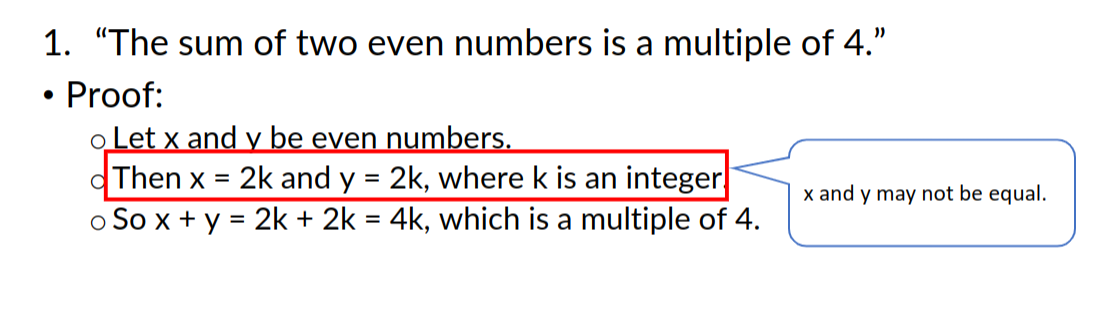
\includegraphics[width=0.7\textwidth]{images/wrongproof-1.png} \\
	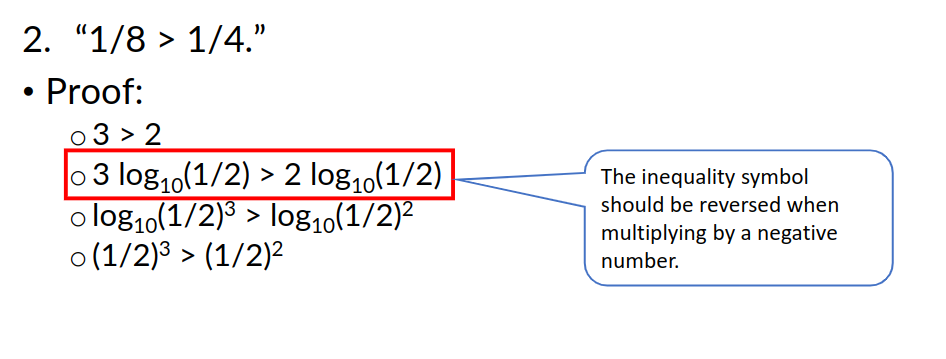
\includegraphics[width=0.7\textwidth]{images/wrongproof-2.png} \\
	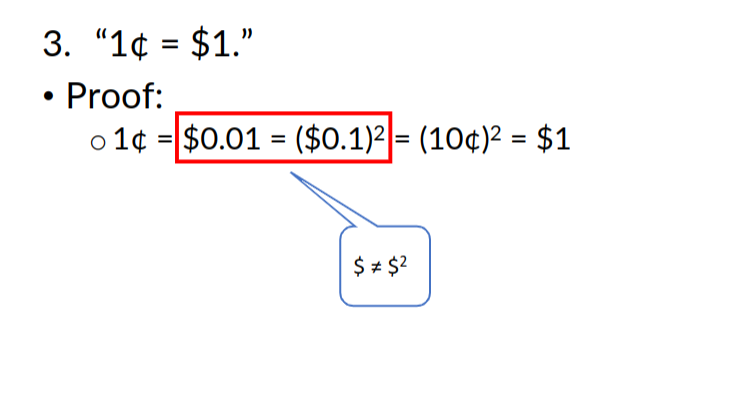
\includegraphics[width=0.7\textwidth]{images/wrongproof-3.png} \\
\end{center}

\pagebreak

\subsection{Proof by Induction}
If you can prove that you can get to $P(n+1)$ from $P(n)$ and also prove that just $P(1)$ is true you can prove $\forall n \ P(n)$ since you're starting at 1 being true and saying anything following it will also be true.
\intextnote[if $P(1)$ is true and $\forall k \ (P(k) \implies P(k+1))$ is true. Then we just follow $P(1) \implies P(2)$, $P(2) \implies P(3)$ and so on...]
\smallbreak \cul{More specifically};
\begin{itemize}[label={}, leftmargin=0.3cm]
	\item Let P be a predicate on positive integers. If\dots
	\begin{enumerate}
		\item \cul{Basis Step:} $P(1)$ is true.
		\item \cul{Inductive Step:} $\forall k \ (P(k) \implies P(k+1))$ is true.
		\begin{itemize}
			\item {\small You prove this by assuming P(k) is true for an arbitrary positive integer k and show that P(k+1) is true.}
		\end{itemize}
	\end{enumerate}
	\item P(n) is true for all positive integers.
\end{itemize}

\bigbreak

\subsubsection*{General Steps / Template}
\begin{enumerate}
	\item Translate into the form “For all $n \ge b, P(n)$” for a fixed integer $b$.
	\item Write out the words “Basis step.” Then show that $P(b)$ is true.
	\begin{itemize}
		\item {\small This is often just a basic sub-in and proving equality.}
	\end{itemize}
	\item Write out the words “Inductive step.”
	\begin{enumerate}
		\item State and clearly identify the inductive hypothesis, in the form “Assume that $P(k)$ is true for an arbitrary (fixed) integer $k \ge b.$”
		\item State what needs to be proved under the assumption that the inductive hypothesis is true, i.e., write out what $P(k + 1)$ says.
		\item Prove $P(k + 1)$ to be true using the assumption P(k) is true.
	\end{enumerate}
	\item Finally, state the conclusion.
\end{enumerate}


\pagebreak

\vspace*{-1cm}
\subsubsection{Examples} \sidenote[Note: there's a ton of additional practice problems on the 9/19 slides if needed.]

\exheader[1] Prove: $1 + 2 + 3 + ... + n = \frac{n(n+1)}{2}$ for any positive integer n.
\begin{itemize}[label={}, leftmargin=0.8cm]
	\item Let $f(n)$ denote $"1+2+3+...+n $
	\item Basis Step $(n=1)$: $ 1 = 1(1+1)/2$ \textcolor{green}{\checkmark}
	\item Inductive Step:
	\begin{itemize}
		\item Assume that for any arbitrary positive integer $k$, $f(k) = \frac{k(k+1)}{2}$
		\item We need to show $f(k+1) = \frac{(k+1)(k+2)}{2}$ \emph{\tiny $\leftarrow$ here we're plugging in $k+1$ in for $k$}
		\item $f(k+1) = 1 + 2 + 3 + ... + k + (k+1) = f(k) + k(k+1) = \frac{k(k+1)}{2} + (k+1) = \frac{(k+1)(k+2)}{2}$
		\item Thus, the statement is true for $k+1$ as well.
	\end{itemize}
\end{itemize}

\bigbreak

\exheader[2] Prove $n^2 > 3n$ for $n \ge 4$ for any positive integer n.
\begin{itemize}[label={}, leftmargin=0.8cm]
	\item Basis step $(n=4)$: we have $4^2 > 3*4$ \textcolor{green}{\checkmark}
	\item Inductive Step:
	\begin{itemize}
		\item Assume that for any arbitrary positive integer $k \ge 4 \ , \ k^2 > 3k$
		\item We need to show that $(k+1)^2 > 3(k+1)$
		\item $(k+1)^2 = k^2 + 2k + 1$ \\
		\begin{tabular}{l l}
			$> 3k + 2k + 1$ & (by the inductive hypothesis) \\
			$\ge 3k + 8 + 1$ & ($k \ge 4$) \\
			$> 3k + 3$ & \\
			$=3(3+1)$ & {\tiny $\leftarrow$ remember this is what we were trying to reduce the RHS to prove $(k+1)^2 > 3(k+1)$}
		\end{tabular}
	\end{itemize}
	\item this completes the proof
\end{itemize}

\bigbreak

\exheader[3] Prove $7^n - 2^n$ is divisible by 5 for \cul{any positive integer $n$}
\begin{itemize}[label={}, leftmargin=0.8cm]
	\item Basis Step: $(n=1)$: we have $7-2=5$, which is divisible by 5.
	\item We need to show that $7^{k+1} - 2^{k+1}$ is divisible by 5
	\item Induction Step:
	\begin{itemize}
		\item Assume that for any arbitrary positive integer $k$, $7^k - 2^k$ is divisible by 5.
		\item We need to show that $7^{k+1} - 2^{k+1}$ is divisible by 5. \\
		\begin{tabular}{rcl}
			$7^{k+1} - 2^{k+1}$ & = & $7*7^k - 2 * 2^k$ \\
			& = & $7 * 7^k - 7 * 2^k + 5 * 2^k$ \\
			& = & $ 7 * (7^k - 2^k) + 5 * 2^k$ \\
			\multicolumn{3}{l}{By the inductive hypothesis, $7 * (7^k - 2^k)$ is divisible by 5,} \\
			\multicolumn{3}{l}{thus $7^{k+1} - 2^{k+1}$ is divisible by 5.}
		\end{tabular}
	\end{itemize}
	\item this completes the proof
\end{itemize} \bigbreak

\pagebreak

\vspace*{-2cm}
\subsection{Strong Induction}
% P(1) does not necessarily mean integer 1- its just the starting element of thje set.
% this method has more assumptions at the start that we can use for the proof as we're assuming a bunch of elements up to P(k) is true.
\horizline
Let P be a predicate on positive integers. If...
\begin{enumerate}
	\item $P(1)$ is true.
	\begin{itemize}[label={\small \faInfoCircle}]
		\item {\small This doesn't necessarily mean integer positive 1. This is wherever the set begins.}
	\end{itemize}
	\item $\forall k (P(1) \land P(2) \land P(3) \land ... \land P(k) \implies P(k+1))$
\end{enumerate}
Then $P(n)$ is true for all positive integers. \\
\horizline 
This method has more assumptions that can be utilized for the proof as it's assuming a bunch of elements \emph{up to} $P(k)$ are true. \smallbreak
The template is nearly identical to our proof by induction.

\subsubsection*{Induction vs Strong Induction}
\begin{itemize}
	\item Induction applies when information about "one position back" is enough for the inductive sterp.
	\item Strong induction applies when you cannot directly prove that $P(k+1)$ is true \cul{just because you know $P(k)$ is true}.
\end{itemize}
\intextnote[Technically, you could use either type for a proof (as their technically equivalent). However, each is significantly easier for different types of proofs.]

\bigbreak
\subsubsection{Examples} \sidenote[Theres also extra excercises for this on the 9/26 slides.]

\bigbreak

% we're going to utilize proof by cases to split k+1 into our two possible conditions
\exheader[1] Prove: every integer $ n > 1$ is prime or a product of primes.
\begin{itemize}[label={}, leftmargin=0.8cm]
	\item Basis step $(n=2)$: 2 is prime.
	\item Inductive step.
	\begin{itemize}
		\item Assume that for any integer $ k \ge 2$, the statement is true for any integer $r$, where $2 \le r \le k$
		\item We need to show that $k+1$ is prime or a product of primes. \\ {\tiny \faInfoCircle we can split it into two the separate conditions using proof by cases.}
		\begin{itemize}
			\item If $k+1$ is prime, we're done.
			\item If $k+1$ isn't prime, then $k+1 = ab$, where $1 < a < k+1$ and $1 < b < k+1$, or equivalently $2 \le a \le k$, $2 \le b \le k$. Based on this assumption, $a$ and $b$ are either prime or the product of primes. Thus, $k+1 = ab$ is a product of primes.
		\end{itemize}
	\end{itemize}
	\item This completes the proof
\end{itemize}

\pagebreak

% method 2 lets us put more stuff in the basis step to avoid so many cases in the inductive step.

\exheader[2] Prove any amount of postage greater than or equal to 8 cents can be built using only 3-cent and 5-cent stamps.
\begin{itemize}[label={}, leftmargin=0.8cm]
	\item Basis Step $(n=8)$: $8 = 3 + 5$
	\item Inductive Step
	\begin{itemize}
		\item Assume that given any positive integer $k \ge 8$, the statement is true for any integer $r$, where $8 \le r \le k$.
		\item Show that $k+1$ can be built using only 3-cent and 5-cent stamps.
		\begin{itemize}
			\item Case 1: $(k+1 = 9)$: $9$ 
			\item Case 2: $(k + 1 = 10)$: $10 = 5 + 5$
			\item Case 3 $(k+ 1 \ge 11)$: $k + 1 = k -2 + 3$. Since $k -2 \ge 8$, $k-2$ can be written as the sum of 3's and 5's. Thus $k+1$ can be written as a sum of 3's and 5's.
		\end{itemize}
	\end{itemize} 
	\item This completes the proof.
\end{itemize}

Thats a lot of cases to go through in the induction steps! Let's do this example again but let's add more base cases in the basis step to avoid adding proof by cases within the inductive step.

\exheader[2.1] Prove any amount of postage greater than or equal to 8 cents can be built using only 3-cent and 5-cent stamps.
\begin{itemize}[label={}, leftmargin=0.8cm]
	\item Basis Step: $(n=8,9,10)$: $8 = 3+5, 9=3+3+3, 10=5+5$
	\item Inductive Step:
	\begin{itemize}
		\item Assume that given any positive integer $k \ge 10$, the statement is true for any integer $r$, where $8 \le r \le k$
		\item Show that $k+1$ can be built using only 3-cent and 5-cent stamps.
		\item \sidenote[this connects our inductive step to our basis step]$k+1 = k-2 + 3$. Since $k -2 \ge 8$, $k-2$ can be written as the sum of 3's and 5's.
		\item Thus, $k+1$ can be written as the sum of 3's and 5's.
	\end{itemize}
	\item This completes the proof.
\end{itemize}

\todo[inline]{TODO: add the tribonacci sequence exercise (its very different than the other examples covered)}


\pagebreak


\section{Sets}
\define[A \textcolor{blue}{\cul{set}} is an unordered collection of objects, which are called the members or elements of the set.]

\subsection{Set Basics}
\begin{itemize}[leftmargin=*, label={}]
	\item A Set is denoted by a capital letter with it's elements contained within curly brackets (comma seperated).
	\begin{itemize}
		\item C = $\{$red, green, blue$\}$
	\end{itemize}
	\item $y \in S$ means that $y$ is a member or an element of $S$, \\ $y \not \in S$ means that $y$ is not a member or an element of S.
	\begin{itemize}
		\item red $\in$ C = $\{$red, green, blue$\}$, but yellow $\not \in$ C.
	\end{itemize}
	\item Sets have no order!
	\begin{itemize}
		\item $\{x,y\}$ is the same as $\{y,x\}$
	\end{itemize}
	\item Each element only occurs once in a set.
	\begin{itemize}
		\item $\{x,x\} \rightarrow {x}$
	\end{itemize}
	\item You can have sets of sets... 
	\begin{itemize}
		\item  $\{\{a, b\}, \{\{b\}\}, \{\{e\}, f\}\}$
	\end{itemize}
\end{itemize} 
\bigbreak

\textbf{Standard Sets} \smallbreak
\begin{tabular}{l c l l}
	$\mathbb{N}$ & = & Set of all nonnegative integers & $\mathbb{N} = \{0,1,2,3,\dots\}$ \\
	$\mathbb{Z}$ & = & Set of all integers & $\mathbb{Z} =  \{\dots , --3, -2, -1, 0, 1, 2, 3 \dots \}$ \\
	$\mathbb{Q}$ & = & Set of all rational numbers & $\frac{1}{2}, \frac{-3}{5}, 16 \dots$ \\
	$\mathbb{R}$ & = & Set of all real numbers & $\pi, e, -9, \sqrt{2} \dots$ \\
	\vspace*{-0.25cm}$\varnothing$& = & Empty set & A set with no elements. \\
	\multicolumn{4}{l}{\tiny \faInfoCircle Note that $\varnothing$  is not the same as $\{\varnothing \}$ }
\end{tabular} \vspace*{-0.5cm} \intextnote[A superscript of "+" restricts a set to its positive elements]
\bigbreak

\textbf{Describing a Set}
\begin{itemize}[leftmargin=*, label={}]
	\item List all the elements.
	\begin{itemize}
		\item Set of all positive even integers: S = $\{2, 4, 6, 8, \dots  \}$
	\end{itemize}
	\item Characterize the property of the elements - \sidenote[this essentially means all $x$ \underline{such that} $P(x)$ is true]$\{x | P(x) \}$
	\begin{itemize}
		\item Set of all positive even integers: \sidenote[you can also use $\land$ instead of "and" here.] S = $\{x | x > 0 \textnormal{ and } x = 2k \textnormal{ for } k \in \mathbb{N} \}$
	\end{itemize}
\end{itemize}

\pagebreak

\textbf{Size of a Set} \\
The \cul{size} or \cul{cardinality} of set S is the number of elements in S denoted by |S|.
\begin{itemize}[leftmargin=*, label={\faAngleRight}]
	\item A is the set of odd positive integers less than 10. |A| = 5.
	\item S is the set of letters in the English alphabet. |S|=26
	\item |$\varnothing$| = 0
	\item |$\mathbb{N}$| = infinity.
\end{itemize}
\bigbreak

\textbf{Power Set} \\
For a set S, the set consisting of \textbf{all} the subsets of S is called the \cul{power set} of S, denoted by $2^{\textnormal{S}}$.
$2^{\textnormal{S}}$ = \{x | x $\subseteq$ S\} \\ The size of $2^{\textnormal{S}}$ is $|2^{\textnormal{S}}| =  2^{|\textnormal{S}|}$
\smallbreak
\cul{Examples} \\
\exheader[1] What is the power set of $\varnothing$?
\begin{itemize}[leftmargin=*, label={}]
	\item $2^\varnothing = \{ \varnothing \}$
	\item $|2^\varnothing| = 2^0 = 1$
\end{itemize}
\exheader[2] Let S = \{a, b, c\}. What is $2^{\textnormal{S}}$?
\begin{itemize}[leftmargin=*, label={}]
	\item The subsets of S:
	\begin{itemize}[leftmargin=*, label={}]
		\item $\varnothing$
		\item \{a\}, \{b\}, \{c\} 
		\item \{a,b\}, \{a,c\}, \{b,c\}
		\item \{a,b,c\}
	\end{itemize}
	\item $2^{\textnormal{S}}$ = \{$\varnothing$, \{a\}, \{b\}, \{c\}, \{a,b\}, \{a,c\}, \{b,c\}, \{a,b,c\}\}
\end{itemize}






\pagebreak

\subsubsection{Examples}
\exheader[1] Describe the following sets by listing their elements:
\begin{enumerate}
	\item \{ x | x $\in \mathbb{N}$ and 3 $<$ x $\le$ 7 \}
	\begin{itemize}[label={\faAngleRight}]
		\item   $\{ 4,5,6,7 \}$
	\end{itemize}
	\item \{ x | x  is a month with exactly 30 days \}
	\begin{itemize}[label={\faAngleRight}]
		\item   \{ April, June, September, November \}
	\end{itemize}
	\item \{ x | x is the capital of the United States \}
	\begin{itemize}[label={\faAngleRight}]
		\item \{ Washington DC \}
	\end{itemize}
\end{enumerate}
\bigbreak
\exheader[2] Describe the following sets by giving a charactering property.
\begin{enumerate}
	\item \{ 1, 4, 9, 16 \}
	\begin{itemize}[label={\faAngleRight}]
		\item \{ x | 1 $\le$ x $\le$ 16 and x = k$^2$ for k $\in \mathbb{N}$ \}
	\end{itemize}
	\item \{ 2, 3, 5, 7, 11, 13, 17, ... \} 
	\begin{itemize}[label={\faAngleRight}]
		\item \{ x | x is prime \}
	\end{itemize}
\end{enumerate}
\bigbreak
\exheader[3] Simplify the descriptions of the following sets:
\begin{enumerate}
	\item A = \{ x | $\exists$ y (y $\in$ \{0,1,2\} and x = y$^3$)\}
	\begin{itemize}
		\item A = \{0,1,8 \}
	\end{itemize}
	\item  B = \{ x | x $\in \mathbb{N}$ and $\exists$ y (y $\in \mathbb{N}$ and x $\le$ y)\}
	\begin{itemize}
		\item B = $\mathbb{N}$
	\end{itemize}
	\item C = \{  x | x $\in \mathbb{N}$ and $\forall$ y (y $\in \mathbb{N} \implies $x $\le$ y)\}
	\begin{itemize}
		\item C = \{ 0 \}
	\end{itemize}
\end{enumerate}

\pagebreak

\subsection{Relationships Between Sets} \label{sec:setrelations}
There are three main set relationships important to this class;
\begin{center}
	\begin{tabular}{c c c}
		Subset & Equal & Proper Subset
	\end{tabular}
\end{center}
\horizline


% making this table gave me cancer
\begin{tabular}{|p{0.14\textwidth}|p{0.28\textwidth}|p{0.5\textwidth}|}
	\hline
	\rowcolor{lightgray} Relationship & Definition & Details \\
	\hline
	\hline
	\rule{0pt}{4ex}\textbf{Subset} & A is a \cul{subset} of B if every element of A is also in element B & \begin{itemize}[leftmargin=*, label={}]
		\item Denoted by: $A \subseteq B$
		\item 
		\item Logical Representation: 
		\item $\forall x (x \in A \implies x \in B)$
	\end{itemize} \\ \hline
	\rule{0pt}{4ex}\textbf{Equal} & Two sets are \cul{equal} if and only if they contain the same elements & \begin{itemize}[leftmargin=*, label={}]
		\item Denoted by A = B
		\item 
		\item Logical Representation: 
		\item $\forall x \ (x \in A \iff x \in B)$
		\item {\tiny or $\forall x \ (x \in A \implies x \in B) \land \forall x \ (x \in B \implies x \in A)$}
		\item 
		\item A = B if and only if A $\subseteq$ B $\land$ B $\subseteq$ A
	\end{itemize} \\ \hline
	\rule{0pt}{4ex}\textbf{Proper Subset} & If A $\subseteq$ B but A $\not =$ B, then A is a \cul{proper subset} of B & \begin{itemize}[leftmargin=*, label={}]
		\item Denoted By A $\subset$ B
		\item 
		\item Logical Representation: 
		\item {\small $\forall x \ (x \in A \implies x \in B) \land  \exists x \ (x \in B \land x \not \in A)$}
	\end{itemize} \\ \hline
\end{tabular}
\bigbreak
\subsubsection*{Example}\sidenote[Theres additional examples and excercises in the 9/28 slides if needed.]

\exheader[1] Let A = \{ 1, 7, 9, 15\}, B = \{7, 9\}, C = \{7, 9, 15, 20\} \\ Then the following statements are all true; \\ 
\begin{tabular}{c  c  c  c  c  c  c}
	B $\subseteq$ C & \{7,9\} $\subseteq$ B & B  $\subset$ A  & \{7\} $\subset$ A & B $\subseteq$ A & $\varnothing \subseteq$ C & 15 $\in$ C \\
\end{tabular} \smallbreak
{\small "$\varnothing \subseteq$ C" is easier to understand if you look at the logical representation: \\ $\forall x (x \in \varnothing \implies x \in C) \ \rightsquigarrow \forall x (\textnormal{F} \implies x \in C)$ \\ Since $\varnothing$ is an empty set, the first part of that implication is false (x cant be in nothing). Meaning the entire statement is true.}
\pagebreak

\subsection{Proving the relationships}
\begin{itemize}[leftmargin=*, label={}]
	\item Prove that $a \in$ A = \{x | P(x)\}
	\begin{itemize}
		\item Show that P($a$) is true.
	\end{itemize}
	\item Prove that A $\subseteq$ B = \{x | P(x)\}
	\begin{itemize}
		\item Pick an arbitrary x $\in$ A and show that P(x) holds.
	\end{itemize}
	\item Prove that A $\subset$ B  = {x | P(x)}
	\begin{itemize}
		\item Prove that A $\subseteq$ B but there exists $a in$ B such that $a \not \in$ A.
	\end{itemize}
	\item Prove that A = B
	\begin{itemize}
		\item A = B means $\forall x (x \in \textnormal{A} \implies x \in \textnormal{B}) \land \forall x (x \in \textnormal{B} \implies x \in \textnormal{A})$
		\item Equivalently, A = B if and only if A $\subseteq$ B $\land$ B $\subseteq$ A.
		\item Prove that A $\subseteq$ B and B $\subseteq$ A.
	\end{itemize}
\end{itemize}
\bigbreak
\subsubsection{Examples}
\bigbreak

\exheader[1] \sidenote[bruh]  Let A = \{ x | x is a multiple of 8\}, and B = \{ x | x is a multiple of 4\}. \\ Prove that A $\subseteq$ B. \\
Proof:
\begin{itemize}[leftmargin=*, label={}]
	\item Let x $\in$ be any arbitrary element.
	\item We need to show that x is a multiple of 4.
	\item Since x is a multiple of 8, x = 8k for some k $\in \mathbb{Z}$
	\item x = 8k = 4*2k = 4m, where m = 2k.
	\item Thus x is a multiple of 4 and x $\in$ B. So A $\subseteq$ B.
	\item (Some numbers, like 12, are multiples of 4 but not 8. So A $\subset$ B)
\end{itemize}
\pagebreak
\exheader[2] Let A = \{ x  | x $\in \mathbb{R}$ and x$^2$-4x+3 = 0\}, and B = \{ x | x $\in \mathbb{N}$ and 1 $\le$ x $\le$ 4\}. \\ Prove that A $\subset$ B. \\
Proof:
\begin{itemize}[leftmargin=*, label={}]
	\item \sidenote[Since there's only two elements, we can just prove each directly.] A can be written as A = {1, 3} {\tiny (just solving for when x satisfies that eq)}
	\item Let x $\in$ A. We need to show that x $\in \mathbb{N}$ and 1 $\le$ x $\le$ 4. Thus x $\in$ B.
	\item If x = 3, then x $\in \mathbb{N}$ and 1 $\le$ x $\le$ 4. Thus x $\in$ B.
	\begin{itemize}
		\item Same idea for 1.
	\end{itemize}
	\item So A $\subseteq$ B.
	\item 2 $\in$ B but $\not \in$ A. So A $\subset$ B.
\end{itemize} 
\bigbreak

\exheader[3] Let A = \{ x | x $\in \mathbb{N}^+$ and x$^2$ < 15\}, and B = \{ x | x $\in \mathbb{N}^+$ and 2x < 7\}. \\ Prove that A = B. \\
\sidenote[We're essentially just showing that the items of each of these sets are the same.]Proof:
\begin{itemize}[leftmargin=*, label={}]
	\item A  $\subseteq$ B
	\begin{itemize}
		\item Let x $\in$ A. Then x can be 1, 2 or 3.
		\item 2x < 7 for any of these three integers.
		\item Thus x $\in$ B and A $\subseteq$ B.
	\end{itemize}
	\item B $\subseteq$ A  
	\begin{itemize}
		\item Let x $\in$ B. Then x can be 1, 2 or 3.
		\item x$^2$ < 15 for any of these three integers.
		\item Thus x $\in$ A and B $\subseteq$ A.
	\end{itemize}
	\item Therefore, we proved that A = B.
\end{itemize} 

\pagebreak

\subsection{Cartesian Product}
The \cul{Cartesian product} of A and B, denoted by A $\times$ B, is defined as A $\times$ B  = \{(x,y) | x $\in$ A $\land$ y $\in$ B \}. \\
{\small \emph{This essentially means all the possible ordered pairs you can make with the items in A and B}}.
\begin{itemize}[leftmargin=*, label={}]
	\item A $\times \varnothing = \varnothing$, $\varnothing \times$ A $= \varnothing$
	\item A $\times$ B = B $\times$ A if 
	\begin{itemize}
		\item A = B or
		\item A or B is $\varnothing$ {\tiny as this would satisfy that first bullet point idea.}
	\end{itemize}
	\item |A $\times$ B| = |A| $\times$ |B|
	\item A$^n$ = A $\times$ A $\times$ ... $\times$ A. (n times) 
	\begin{itemize}
		\item A$^2$ = A $\times$ A
		\item A$^3$ = A $\times$ A $times$ A.
	\end{itemize} {\tiny \vspace*{-0.5cm} Note that these multi-products creates an n-tuple set $(\_,\_,\_,...)$}
\end{itemize}
\begin{tabular}{c c c c}
	In general, & (A $\times$ B) $\times$ C  \ $\not =$ & A $\times$ (B $\times$ C) \ $\not =$ & A $\times$ B $\times$ C. \\
	& $((\_,\_),\_)$ & $(\_,(\_,\_))$ & $(\_,\_,\_)$
\end{tabular}
\\ {\tiny \emph{These would only be equal when A, B, or C = $\varnothing$}}
\bigbreak
\textbf{Examples}
\smallbreak
\exheader[1] A = \{1,2\}, B = \{2,4\}
\begin{itemize}[label={}]
	\item A $\times$ B = \{(1,2), (1,4), (2,2), (2,4)\}
	\item B $\times$ A = \{(2,1), (4,1), (2,2), (4,2)\}
\end{itemize}
\smallbreak
\exheader[2] A = \{1,2\}
\begin{itemize}[label={}]
	\item A$^2$ = \{(1,1), (1,2), (2,1), (2,2)\} 
	\item A$^3$ = \{(1,1,1), (1,1,2), (1,2,1), (1,2,2), (2,1,2), (2,2,1) (2,2,2)\}
\end{itemize}



\pagebreak

\subsection{Set Operations}
\begin{center}
{\small
\begin{tabular}{c c c c}
	Union & Intersection & Set Difference & Complement
\end{tabular}
}
\end{center}
\bigbreak

Before each of these operations is introduced, let's look at the \cul{Venn Diagram} as it is an important tool to demonstrate what these operations are "pulling" from the sets. \\
A set S is called the \cul{universal set} if it contains all objects \sidenote[If we're considering all real numbers then S = $\mathbb{R}$. If we're considering students at Mines, then the set is all students at Mines.]under consideration \smallbreak
A Venn diagram is used to visualize all possible relations of sets. All within this universal set S (depicted as a box around the Venn Diagram). Reference the image next to every set operations description for a quick visualization of the set relation.
\intextnote[Note that while Venn diagrams are helpful for illustrating an operation, \\ \cul{they should not be used for a proof}]

\bigbreak
\horizline


% THIS IS THE OLD BROKEN WAY OF DOING IT THAT BREAKS INDENTATIOIN - KEEPING FOR REF.
%\begin{wrapfigure}{R}{0.25\textwidth} %this figure will be at the right
%    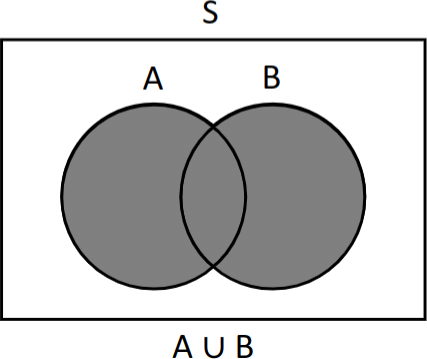
\includegraphics[width=0.25\textwidth]{images/venn/AuB.png}
%\end{wrapfigure}
%
%{\small The union of A and B, denoted by A $\cup$ B is $\{x | x \in $ A $ \lor \ x \in $ B $\}$} \vspace*{-0.25cm} \\ {\tiny All the elements in A combined with all the elements in B} \vspace*{-0.25cm} \smallbreak
%\cul{Example}
%\begin{itemize}[label={}]
%	\item Let A = \{1, 3, 5, 7, 9\} and B = \{3, 5, 6, 10, 11\}
%	\item Then A $\cup$ B = \{1, 3, 5, 6, 7, 9, 10, 11\}
%\end{itemize}


\subsubsection*{Union} 
{\small The union of A and B, denoted by A $\cup$ B is $\{x | x \in $ A $ \lor \ x \in $ B $\}$} \vspace*{-0.25cm} \\ {\tiny All the elements in A combined with all the elements in B} \vspace*{-0.25cm} \smallbreak
\begin{minipage}[t]{0.7\linewidth}
\cul{Example}
\begin{itemize}[leftmargin=*, label={}]
	\item Let A = \{1, 3, 5, 7, 9\} and B = \{3, 5, 6, 10, 11\}
	\item Then A $\cup$ B = \{1, 3, 5, 6, 7, 9, 10, 11\}
\end{itemize}
\end{minipage}
\begin{minipage}[t]{0.25\linewidth}
    \centering
    \strut\vspace*{-\baselineskip}\newline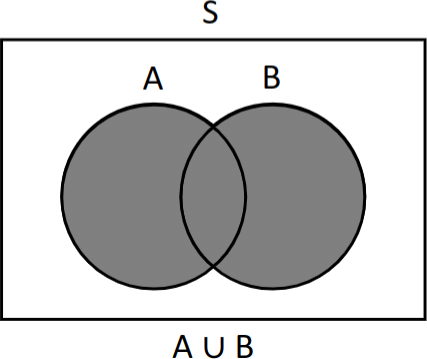
\includegraphics[width=\linewidth]{images/venn/AuB.png}
  \end{minipage}

\bigbreak

\subsubsection*{Intersection} \label{sec:intersectiondef}
{\small The intersection of A and B, denoted by A $\cap$ B is $\{x | x \in $ A $ \land \ x \in $ B $\}$} \vspace*{-0.25cm} \\ {\tiny The elements that are in both A and B} \vspace*{-0.25cm} \smallbreak
\begin{minipage}[t]{0.7\linewidth}
	\cul{Example}
	\begin{itemize}[leftmargin=*, label={}]
		\item Let A = \{1, 3, 5, 7, 9\} and B = \{3, 5, 6, 10, 11\}.
		\item Then A $\cap$ B = \{3,5\}
	\end{itemize}
\end{minipage}
\begin{minipage}[t]{0.25\linewidth}
	\centering
    \strut\vspace*{-\baselineskip}\newline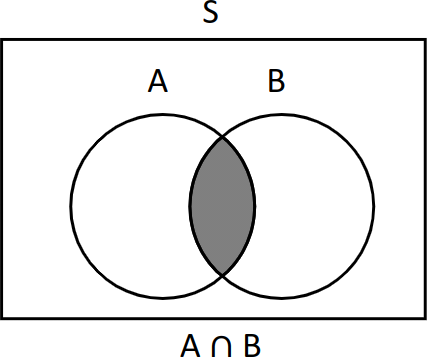
\includegraphics[width=\linewidth]{images/venn/AnB.png}
\end{minipage}

\pagebreak


\subsubsection*{Set Difference}
{\small The set difference of A and B, denoted by A - B, is $\{x|x \in $ A $ \land \ x \not \in $ B $ \}$} \vspace*{-0.25cm} \\ {\tiny The elements that are in A but not in B} \vspace*{-0.05cm} \\
\begin{minipage}[t]{0.7\linewidth}
	{\small Note: A - B = A - (A $\cap$ B)}
	\smallbreak
	\cul{Example}
	\begin{itemize}[leftmargin=*, label={}]
		\item Let A = \{1, 3, 5, 7, 9\} and B = \{3, 5, 6, 10, 11\} 
		\item Then A - B = \{1, 7, 9\}
	\end{itemize}
\end{minipage}
\begin{minipage}[t]{0.25\linewidth}
	\centering
    \strut\vspace*{-\baselineskip}\newline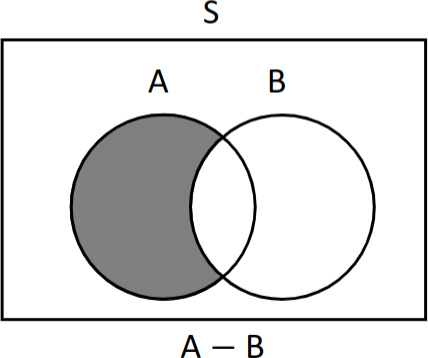
\includegraphics[width=\linewidth]{images/venn/A-B.png}
\end{minipage}


\subsubsection*{Complement}
{\small Let A $\subseteq$ S. The complement of A, denoted by A$'$, is $\{x|x \in $ S $ \land \ x \not \in $ A $\}$} \vspace*{-0.25cm} \\ {\tiny The set of everything \cul{not} in A} \vspace*{-0.25cm} \smallbreak
\begin{minipage}[t]{0.7\linewidth}
\cul{Example}
	\begin{itemize}[leftmargin=*, label={}]
		\item S = $\mathbb{N}$
		\item A = $\{x | x \in \mathbb{N} \land x = 2k $ for $ k \in \mathbb{N}\}$
		\item A$'$ = $\{x | x \in \mathbb{N} \land x = 2k + 1$ for $ k \in \mathbb{N}\}$
	\end{itemize}
\end{minipage}
\begin{minipage}[t]{0.25\linewidth}
	\centering
    \strut\vspace*{-\baselineskip}\newline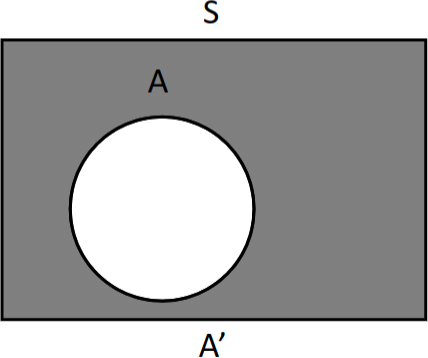
\includegraphics[width=\linewidth]{images/venn/Ap.png}
\end{minipage}

\subsubsection*{Set Difference and Intersection}
\begin{minipage}[t]{0.7\linewidth}
	Two sets A and B are \cul{disjoint} if A $\cap$ B = $\varnothing$. \vspace*{-0.25cm} \\ {\tiny Meaning they have no elements in common} \vspace*{-0.25cm} \smallbreak
	If A and B are disjoint, then A - B = A and B - A = B \smallbreak
	For any A $\subseteq$ S, B $\subseteq$ S, A - B and B - A are disjoint.
\end{minipage}
\begin{minipage}[t]{0.25\linewidth}
	\centering
    \strut\vspace*{-\baselineskip}\newline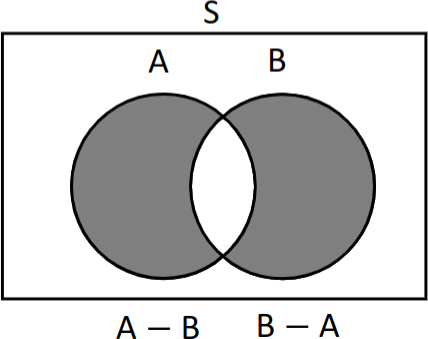
\includegraphics[width=\linewidth]{images/venn/A-B B-A.png}
\end{minipage}



\subsubsection*{Set Difference and Complement}

{\small The set difference can be rewritten as $\{x | x \in $ A $ \land \ x \in $ B$'\}$. Therefore, A - B = A $\cap$ B$'$}
\begin{figure}[!h]
	\centering
	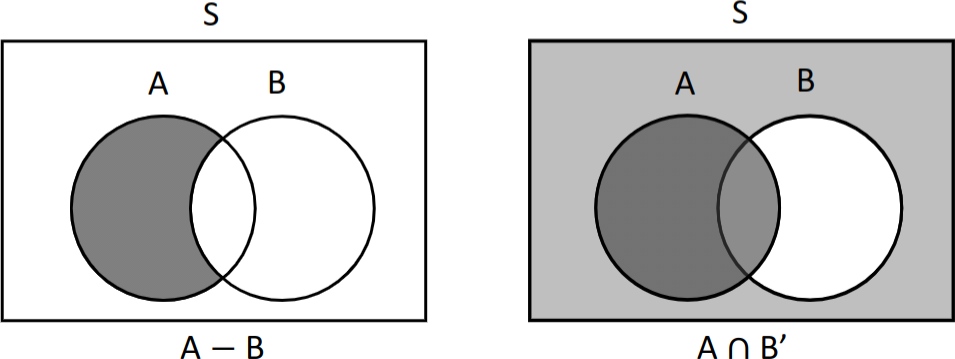
\includegraphics[width=0.60\textwidth]{images/venn/diffandcomp.png}	
\end{figure} \vspace*{-0.25cm} \\
{\tiny \emph{The darkest shaded part is what is actually included by the operation A $\cap$ B$'$, the other shades are the "layers" of each operation}}

\pagebreak

\subsubsection{Proving Relations Involving Set Operations} 
\vspace*{-0.3cm}
{\small (Examples)} \\
In general, its good to start by looking at the Venn Diagram for visually understanding why a statement is true, and deriving the formal proof from there.

\bigbreak

\exheader[1] Prove that A $\cup$ B $\subseteq$ A \\
{\small \emph{We need to show that for some arbitrary element in A, that element is also in B. \\ $\rightsquigarrow \ x \in A \implies x \in B$ }}
\\ Proof:
\begin{itemize}[leftmargin=*, label={}]
	\item Let x be an arbitrary member of A $\cap$ B. \\
	\begin{tabular}{l l l}
		$x \in A \cap B$ & $\implies$ &  $x \in A \land x \in B$ {\tiny \emph{using the definition of intersection here}} \\
		& $\implies$ & $x \in A$ {\tiny \emph{Treat $x \in A \land x \in B$ as $P \land Q$ and use Simplification Inf' Law}}
	\end{tabular}
	\item Therefore, A $\cap$ B $\subseteq$ A. {\tiny \emph{By the definition of subset relation \\ Or intuitively we've shown that any x in A $\cap$ B is also in just A}}
\end{itemize}

\bigbreak

\exheader[2] Prove that C $\subseteq$ A and C $\subseteq$ B if and only if C $\subseteq$ A $\cap$ B. \vspace*{-0.2cm}
\\ {\tiny \emph{Remember we can break $P \iff Q$ into $(P \implies Q) \land (Q \implies P)$ where $P$ is "C $\subseteq$ A and C $\subseteq$ B" and Q is "C $\subseteq$ A $\cap$ B"}} 
\smallbreak Proof:
\smallbreak First we need to prove the "only if" {\tiny \emph{($P \implies Q$)}} part:
\begin{itemize}[leftmargin=*, label={}]
	\item Let x be an arbitrary member of C. \\
	\begin{tabular}{l l l}
		$ x \in C $ & $\implies$ & $x \in A \land x \in B$ {\tiny \emph{Since C $\subseteq$ A and C $\subseteq$ B}} \\
		& $\implies$ & $x \in A \cap B$ {\tiny \emph{Reference the \hyperref[sec:intersectiondef]{intersection definition}.}}
	\end{tabular}
\end{itemize} \smallbreak
Now we prove the "If" {\tiny \emph{$Q \implies P$}} part:
\begin{itemize}[leftmargin=*, label={}]
	\item Let x be an arbitrary member of C. \\
	\begin{tabular}{l l l}
		$ x \in C$ & $\implies$ & $x \in A \cap B$ {\tiny \emph{From hypothesis "C $\subseteq$ A $\cap$ B"}} \\
		& $\implies$ & $x \in A \land x \in B$ {\tiny \emph{From the \hyperref[sec:intersectiondef]{intersection definition} again.}}
	\end{tabular}
	\item Therefore, $C \subseteq A \land C \subseteq B$ {\tiny \emph{Reference the logical rep' of a subset \hyperref[sec:setrelations]{(from the table)}}}
\end{itemize}

\pagebreak

\exheader[3] Prove that $2^A \cap 2^B = 2^{A \cap B}$
\\ {\small \emph{You can prove two sets to be equal by proving Left $\subseteq$ Right and Right $\subseteq$ Left \\ $\rightsquigarrow$ \ Prove $2^A \cap 2^B \subseteq 2^{A \cap B}$ and \ $2^{A \cap B} \subseteq 2^A \cap 2^B$}}
\\ Proof:
\smallbreak $2^A \cap 2^B \subseteq 2^{A \cap B}$ \vspace*{-0.25cm}
\begin{itemize}[leftmargin=*, label={}]
	\item Let x be an arbitrary member of $2^A \cap 2^B$. \\
	\begin{tabular}{l l l}
		$x \in 2^A \cap 2^B$ & $\implies$ & $x \in 2^A \land x \in 2^B$ \\
		& $\implies$ & $x \subseteq A \land x \subseteq B$ {\tiny \emph{Ref Power Set Definition, If x is a member of a power set, its also a member of the main set}} \\
		& $ \implies $ & $x \subseteq A \cap B$ {\tiny \emph{Intersection Def-kinda ref examples above}} \\
		& $ \implies $ & $x \in 2^{A \cap B}$ {\tiny\emph{Reverse use of the same Power Set Def, if x is a member of this set, its also a member of the power set}}
	\end{tabular}
	\item Therefore $2^A \cap 2^B \subseteq 2^{A \cap B}$
\end{itemize} \smallbreak

$2^{A \cap B} \subseteq 2^A \cap 2^B$ \vspace*{-0.25cm}
\begin{itemize}[leftmargin=*, label={}]
	\item Let x be an arbitrary member of $2^{A \cap B}$ \\
	\begin{tabular}{l l l}
		$ x \in 2^{A \cap B}$ & $\implies$& $x \subseteq A \cap B$ \\
		& $\implies$ & $x \subseteq A \land x \subseteq B$ \\
		& $\implies$ & $x \in 2^A \land x \in 2^B$
	\end{tabular}
	\item Therefore, $2^{A \cap B} \subseteq 2^A \cap 2^B$.
\end{itemize}

\bigbreak
% hard to show set empty - direct proof bad option
% contraposition - would make A is empty, same issue
% proof by contradiction best option
\exheader[4] Prove that if $A \not = \varnothing$ and $A \cap B = A - B$, then $B = \varnothing$
\\ {\small \emph{Both a direct proof and proof by contraposition lead to you trying to prove a set is empty, which is very difficult. So the best option is proof by contradiction}}
\smallbreak Proof: 
\\ Assume to the contrary that {\small $A \not = \varnothing$, $A \cap B = A - B$ and $B \not =\varnothing$}

	\cul{Case 1: $A \cap B = \varnothing$ ($A \cap B$ is empty)}
	\begin{itemize}[label={}]
		\item $A \cap B = A - B$ (from second assumption)
		\item $A - B = A$ (ref "set difference and intersection" notes.)
		\item All combining to $ A \cap B = \varnothing = A - B = A \not = \varnothing$ 
		\item "$\varnothing \not = \varnothing$", We have a contradiction.
	\end{itemize}
	\cul{Case 2: $A \cap B \not = \varnothing$}
	\begin{itemize}[label={}]
		\item Let x be any element in A $\cap$ B. \\
		\begin{tabular}{l l l}
			$x \in A \cap B$ & $\implies$ & $x \in A - B$ {\tiny \emph{(from $A \cap B = A - B$)}} \\
			& $\implies $ & $x \not \in B$ {\tiny \emph{(defn of a set difference)}}
		\end{tabular}
		\item This is a contradiction, since $x \in A \cap B$ implies that $x \in B$
	\end{itemize}

\pagebreak

\subsection{Set Identities}
\define[Set identities are a group of laws that can be used to prove equality between sets. They are all equalities, involving union, intersection, difference, and complementation, that are \cul{always true} for all subsets of a given set S.]

\begin{tabular}{ |p{0.45\linewidth}|p{0.5\linewidth}|}
	\hline
	\rowcolor{lightgray} \multicolumn{2}{|c|}{Set Identities} \\
	\hline
	\hline
	\smallbreak Identity Laws & \begin{itemize}[leftmargin=*, label={}]
		\item A $\cup \ \varnothing =$ A
		\item A $\cap$ S = A \vspace*{-0.3cm}
	\end{itemize}\\ \hline
	\smallbreak Domination Laws & \begin{itemize}[leftmargin=*, label={}]
		\item A $\cup$ S $=$ S 
		\item A $\cap \ \varnothing = \varnothing$ \vspace*{-0.3cm}
	\end{itemize} \\ \hline 
	\smallbreak Idempotent Laws & \begin{itemize}[leftmargin=*, label={}]
		\item A $\cup$ A = A
		\item A $\cap$ A = A \vspace*{-0.3cm}
	\end{itemize} \\ \hline 
	\smallbreak Complementation Law & \begin{itemize}[leftmargin=*, label={}]
		\item \vspace*{0.15cm} (A$'$)$'$ = A
		%\item \vspace*{-0.3cm} % empty item so the spacing looks better lol 
	\end{itemize} \\ \hline 
	\smallbreak Commutative Laws & \begin{itemize}[leftmargin=*, label={}]
		\item A $\cup$ B = B $\cup$ A 
		\item A $\cap$ B = B $\cap$ A \vspace*{-0.3cm}
	\end{itemize} \\ \hline 
	\smallbreak Associative Laws & \begin{itemize}[leftmargin=*, label={}]
		\item (A $\cup$ B) $\cup$ C = A $\cup$ (B $\cup$ C)
		\item (A $\cap$ B) $\cap$ C = A $\cap$ (B $\cap$ C) \vspace*{-0.3cm}
	\end{itemize} \\ \hline
	\smallbreak Distributive Laws & \begin{itemize}[leftmargin=*, label={}]
		\item A $\cup$ (B $\cap$ C) = (A $\cup$ B) $\cap$ (A $\cup$ C)
		\item A $\cap$ (B $\cup$ C) = (A $\cap$ B) $\cup$ (A $\cap$ C) \vspace*{-0.3cm}
	\end{itemize} \\ \hline
	\smallbreak DeMorgan's Laws & \begin{itemize}[leftmargin=*, label={}]
		\item (A $\cap$ B)$'$ = A$'$ $\cup$ B$'$
		\item (A $\cup$ B)$'$ = A$'$ $\cap$ B$'$ \vspace*{-0.3cm}
	\end{itemize} \\ \hline
	\smallbreak Absorption Laws & \begin{itemize}[leftmargin=*, label={}]
		\item A $\cup$ (A $\cap$ B) = A
		\item A $\cap$ (A $\cup$ B) = A \vspace*{-0.3cm}
	\end{itemize} \\ \hline
	\smallbreak Complement Laws & \begin{itemize}[leftmargin=*, label={}]
		\item A $\cup$ A$'$ = S 
		\item A $\cap$ A$'$ = $\varnothing$ \vspace*{-0.3cm}
	\end{itemize} \\ \hline
\end{tabular}

\todo[inline]{TODO: Add venn diagram images (pictures including the rule is fine)}

\pagebreak

\subsubsection{Proving Identities}
\vspace*{-0.3cm}
{\small (Examples)} \\
\smallbreak

\exheader[1] Prove that A $\cup$ (B $\cap$ C) = (A $\cup$ B) $\cap$ (A $\cup$ C) \\ Proof: \\
We need to prove:
\begin{itemize}[leftmargin=*, label={}]
	\item A $\cup$ (B $\cap$ C) $\subseteq$ (A $\cup$ B) $\cap$ (A $\cup$ C)
	\item (A $\cup$ B) $\cap$ (A $\cup$ C) $\subseteq$ A $\cup$ (B $\cap$ C)
\end{itemize}
Prove that A $\cup$ (B $\cap$ C) $\subseteq$ (A $\cup$ B) $\cap$ (A $\cup$ C):
\begin{itemize}[label={}]
	\item Let x be an arbitrary member of A $\cup$ (B $\cap$ C) \\
	\begin{tabular}{l l l}
		$x \in A \cup (B \cap C)$  & $\implies$ & $x \in A \lor x \in (B \cap C)$ \\
		& $\implies$ & $x \in A \lor (x \in B \land x \in C)$ \\
		& $\implies$ & $(x \in A \lor x \in B) \land (x \in A \lor x \in C)$ \\
		& $\implies$ & $(x \in A \cup B) \land (x \in A \cup C)$ \\
		& $\implies$ & $x \in (A \cup B) \cap (A \cup C)$
	\end{tabular}
\end{itemize}
Prove that (A $\cup$ B) $\cap$ (A $\cup$ C) $\subseteq$ A $\cup$ (B $\cap$ C)
\begin{itemize}[label={}]
	\item Let x be an arbitrary member of (A $\cup$ B) $\cap$  (A $\cup$ C). \\
	\begin{tabular}{l l l}
		$x \in (A \cup B) \cap (A \cup C)$ & $\implies $ & $(x \in A \cup B) \land (x \in A \cup C)$ \\
		& $\implies$ & $(x \in A \lor x \in B) \land (x \in A \lor x \in C)$ \\
		& $\implies$ & $x \in A \lor (x \in B \land x \in C)$ \\
		& $\implies$ & $x \in A \lor x \in (B \cup C)$ \\
		& $\implies$ & $x \in A \cup (B \cap C)$
	\end{tabular}
\end{itemize}


\todo[inline]{TODO: Add exercises if needed}


\pagebreak

\section{Recursion}
\define[A \cul{recursive definition}  is a definition in which the object being defined appears as part of the definition]

There are two parts of a recursive definition:
\begin{itemize}[leftmargin=*, label={}]
	\item Basis Step: some simple cases of the object being defined are explicitly given (end of the recursion).
	\item Recursive step: New cases of the object being defined are given in terms of "previous" or "simpler" cases.
\end{itemize}
The relation in the recursive step is called the \cul{recurrence relation}.
\smallbreak
\textbf{Examples}
\begin{enumerate}
	\item Give a recursive definition for the ancestors of James. \\ Recursive Definition:
	\begin{itemize}
		\item Basis Step: James' parentsd are ancestors of James.
		\item Recursive Step: The parents of James' ancestors are ancestors of James.
	\end{itemize}
	\item Give a recursive defintion of the exponentiation operation $a^n$ on a nonzero real number $a$, where $n$ is a nonnegative integer. \\ Recursive Definition:
	\begin{itemize}
		\item Basis Step: $a^0 = 1$
		\item Recursive Step: $a^n = (a^n-1)a$ for $n \ge 1$
	\end{itemize}
\end{enumerate}

\pagebreak

\subsection{Sequences}
A \cul{sequence} is an ordered list of elements, denoted by, \begin{center}$S_1, S_2, S_3, ...$\end{center}
Where $S_k$ denotes the $k$th element in the sequence. \\ Examples:
\begin{itemize}[leftmargin=*, label={}]
	\item 1,2,3,5,8 is a sequence of 5 elements.
	\item 1,3,9,27,81,...,3$^n$,... is an infinite sequence. 
\end{itemize}

\subsubsection*{Summations}
Given the sequence $a_1,a_2,a_3,...a_n$ we use the notation 
{\Large
\[
	\sum_{i=m}^{n} a_i
\]
}
{\small to denote the sum of the terms $a_m, a_{m+1}, ..., a_n$. Read as "the sum from $i = m$ to $i = n$ of a$_i$"} \\ Examples: 
\begin{itemize}[leftmargin=*, label={}]
	\item $1+2+...+n = \sum_{i=1}^{n}i$
	\item $\sum_{j=1}^{5}=1^2+2^2+3^2+4^2+5^2$
\end{itemize}

\bigbreak
\bigbreak

\subsubsection*{Recursively Defined Sequences}
A sequence might be defined recursively by explicitly naming the first value (or the first few values) and then defining later values n terms of previous values. \smallbreak
\textbf{Examples} \\
\exheader[1] Sequence $F_n$
\begin{itemize}[leftmargin=*, label={}]
	\item Basis Step: $F_1 = 1, F_2 = 1$ 
	\item Recursive step: $F_n = F_{n-1} + F_{n-2}$ for $n > 2$
\end{itemize}
The sequence is 1,1,2,3,5,8,13,21,... Otherwise known as the Fibonacci sequence.

\bigbreak

\exheader[2] Give a recursive definition of the sequence $a_1, a_2, a_3, ...,$ where $a_n=4n-2$ for $n \ge 1$
\begin{itemize}[leftmargin=*, label={}]
	\item Basis Step: $a_1 = 2$
	\item Recursive step: $a_n = a_{n-1}+4$ for $n \ge 2$
\end{itemize}

\todo[inline]{TODO (if needed): Add Fibbonacci Proof.}

\pagebreak

\subsubsection*{Recursively Defined Sets}
A set might be defined recursively by explicitly describing one or more \cul{simple elements} and then defining other elements \cul{in terms of existing simpler elements} in the set. \bigbreak

\exheader[1] The set of positive integers, denoted by $\mathbb{N}^+$ has the recursive definition:
\begin{itemize}[leftmargin=*, label={}]
	\item 1 is $\mathbb{N}^+$
	\item If n is in $\mathbb{N}^+$, then n+1 is in $\mathbb{N}^+$
\end{itemize}

\bigbreak

\exheader[2] Give a recursive definition of the set S of positive integers that are multiples of 5.
\begin{itemize}[leftmargin=*, label={}]
	\item Basis Step: $5 \in S$
	\item Recursive step: If $x \in S$, then $x+5 \in S$ (or $x \in S \implies x + 5 \in S$)
\end{itemize}

\bigbreak

\exheader[3] Give a recursive definition of the set of strings, that, is $\sum^* = ${"", "a", "amigien", "words", "school", "ziemg"...} \\ 
Notations: 
\begin{itemize}[leftmargin=*, label={}]
	\item $\lambda$ is the empty string "".
	\item $\Sigma$ is the set of all letters {a,b,c...}
	\item Let $x \in \Sigma^*$ and $y \in \Sigma^*$. xy is the concatenation of x and y.
\end{itemize}
Recursive Definition:
\begin{itemize}[leftmargin=*, label={}]
	\item Basis step: $\lambda \in \Sigma^*, x \in \Sigma^*$ where $x \in \Sigma$
	\item Recursive step: $x \in \Sigma^* \land y \in \Sigma^* \implies xy \in \Sigma^*$
\end{itemize}
\bigbreak
\todo[inline]{There's a ton of exercises and further descriptions of the examples in the videos and slides, add those if needed!}

\pagebreak

\subsubsection*{Recursively Defined Sequence}

\subsection{Closed Form Solution}


\textbf{Intro/Motivation} \smallbreak
Consider the following recursively defined sequence;
\begin{itemize}[leftmargin=*, label={}]
	\item Basis step: $S_1 = 2$
	\item Recursive Step: $S_n = 2S_{n-1}$ for $n \ge 2$
	\item $S$ would be the sequence 2,4,8,16,32 {\tiny \emph{notice a pattern here?}}
\end{itemize}
If you were to represent this sequence in code you'd get something like one of these;

\begin{minipage}[t]{0.5\linewidth}
\begin{verbatim}
int S_prev = 2;
for(int i = 2; i <= n; ++i)
{
    S = 2*S_prev;
    S_prev = S;
}
\end{verbatim}
\end{minipage}
\begin{minipage}[t]{0.5\linewidth}
\begin{verbatim}
	int CompSn(int n)
{
    if(n == 1)
        return 2;
    return 2*CompSn(n-1);
}
\end{verbatim}
\end{minipage}

Note that both of these would be O(n), quite a gross time complexity for something with a clear trend. \\
Looking back at our sequence $S_n$ is just $2^n$! In other words, our two sets of code could be replaced with an \sidenote[This time complexity comes from the implementation of pow] O($\log n$) \verb|int Sn = pow(2,n)|. 
\bigbreak
\bigbreak

\pagebreak


\subsubsection*{Definitions}

What we did above is an example of finding/solving the \textbf{closed-form solution}. \\ An equation, where we can substitute values and get the output value back directly, is called a closed-form solution. \\
Another example would be $x = \frac{-b \pm \sqrt{b^2 -4ac}}{2a}$ as the closed-form solution to $ax^2 + bx + c = 0$. \\ Note that an algorithm is \cul{not} a closed-form solution because you cannot get an output value directly.
\\ Not all kinds of recurrence relations can be solved.

\bigbreak

\begin{itemize}[leftmargin=*, label={}]
	\item A recurrence relation for a sequence $S_1, S_2, S_3, ...$ is a \cul{linear recurrence relation} if $S_n$ is a linear function of the previous elements.
	\begin{itemize}
		\item The \cul{general linear recurrence relation} has the form: \\ $S_n = f_1(n) S_{n_1} + f_2 S_{n-2} + ... f_k S_{n-k} + g(n)$ \\ where $1 \le k \le n-1$, the $f_i$'s and g \cul{can} be expressions involving n.
		\item The recurrence relation has \cul{constant coefficients} if the $f_i$'s are all constants.
	\end{itemize}
	\item
	\item A recurrence relation is \cul{first-order} if the $n$th element depends only on the $(n-1)$th element. \\ {\tiny \cul{examples:}}
	\small
	\begin{tabular}{l l}
		$S_n$ = $2S_{n-1}$ & Linear, first-order. \\
		$F_n = F+{n-1} + F_{n-2}$ & Linear but not first order. \\
		$S_n = S_{n-1} S_{n-2}$ & Not Linear.
	\end{tabular} 
	\begin{itemize}
		\item The general form solution with a constant coefficient {\large $S_n = cS_{n-1} + g(n)$} for $n \ge 2$ can be expanded k times to look like; \\ $c^k S_{n-k} + c^{k-1}g(n-(k-1)) + ... + cg(n-1) + g(n)$ \\
		This series of expansions will stop when $n-k =1$ So we can say that $k = n-1$. Giving us a better solution of $c^{n-1} S_1 + c^{n-2} g(2) + ... + cg(n-1) + c^0 g(n)$. Finally we can simplify this further by using summation notation; \\
		{\large $S_n = c^{n-1} S_1 + \sum_{i=2}^{n} c^{n-i} g(i)$} \\ 
		So to solve for linear first-order, constant coeff recurrence relations you must identify $c$ and $g(n)$ and plug into the form above. You can identify $c$ and $g(n)$ by arranging the recurrence relation into the $S_n = cS_{n-1} + g(n)$ form.
	\end{itemize}
\end{itemize}

\normalsize

\pagebreak

\subsubsection*{Examples}

\exheader[1] Solve $S_n = 2S_{n-1} + 3$ for $n \ge 2$  with $S_1 = 4$
\begin{itemize}[leftmargin=*, label={}]
	\item Match and identify c and g(n) \\ $c=2$ \quad $g(n) = 3$
	\item Substitute in $S_n = c^{n-1} S_1 + \sum_{i=2}^{n} c^{n-i} g(i)$ \\
	\begin{tabular}{l l l}
		$S_n$ & $=$ & $2^{n-1} * 4 + \sum_{i=2}^{n} 2^{n-1} * 3$ \\
		& $=$ & $2^n+1 + 3(2^{n-1} -1)$ {\tiny We're Simplifying the summation here by using the identity: $1+2+2^2+...+2^m = 2^{m+1} -1$ where $m = n-2$}
	\end{tabular}
\end{itemize}

\bigbreak

\exheader[2] Solve $T_n = T_n-1 + (n+1)$ for $n \ge 2$ with $T_1 = 2$
\begin{itemize}[leftmargin=*, label={}]
	\item Match and identify c and g(n) \\ $c=1$ \quad $g(n) = n+1$
	\item Substitute \\
	\begin{tabular}{l l l}
		$T_n$ & $=$ & $1^{n-1} * 2 + \sum_{i=2}^{n} 1^{n-i} (i +1)$ \\
		& $=$ & $2 + (3+4+...+(n+1))$ \\
		& $=$ & $\frac{(n+1)(n+2)}{2} -1$ {\tiny We're simplifying using the identity: $1+2+3+...+m = \frac{m(m+1)}{2}$}
	\end{tabular}
\end{itemize}


\pagebreak

\section{Counting}

\subsection{Basics}
\define[\cul{Counting} is the process of determining the number of a set of objects with certain properties. \\ \cul{For example}; \begin{itemize}
	\item The number of students in a classroom
	\item Number of phone numbers in the US  
	\item Least number of students out of 15 born on the same day of the week. \vspace*{-0.5cm}
\end{itemize}\quad]

Counting problems can be very difficult and now obvious to solve. The general technique and solution to counting problems is to \cul{divide and conquer}, simplifying the problem by decomposing it. \\
More specifically, we'll be working with four counting principles;
\begin{center}
	{\small 
\begin{tabular}{c c}
	Multiplication Principle & Addition Principle \\
	Principle of inclusion and exclusion & Pigeonhole principle
\end{tabular}
}
\end{center}

\pagebreak

\subsubsection{Multiplication Principle} 
Suppose that a task can be broken down into a sequence of two
independent steps. If there are $n_1$ ways to do the first step and for
each of ways of doing the first step, there are $n_2$ ways to do the
second step, then there are $n_1n_2$ ways to complete the task. \smallbreak
\cul{Set Representation:} Let $A$ and $B$ denote the set of ways to do the first and second step, respectively. Then $|A \times B| = |A| \cdot |B|$
\smallbreak
\cul{Generalization:} If a task can be broken into a sequence of $m$ \textcolor{red}{independent} steps, where step $i$ can be done in $n_i$ ways, $i = 1,2,...,m$, then the number of ways to complete the task is;  \sidenotenl[Note that $\prod$ is the product of everything in the sequence.]
	\[ \prod_{i=i}^{\mathclap{m}} n_i = n_1 \cdot n_2 \cdot n_3 \cdot ... \cdot n_m \]
\bigbreak

\subsubsection*{Examples}

\exheader[1] The chairs of an auditorium are to be labeled with an uppercase English letter followed by a positive integer not exceeding 100. What is the largest number of chairs that can be labeled differently?
\begin{itemize}[leftmargin=*, label={}]
	\item Label a chair by a sequence of 2 steps: \\
	\begin{tabular}{l l l}
		Step 1: & Choose an uppercase English letter & 26 ways \{A,B,C,...,Z\} \\
		Step 2: & Choose a positive integer $\le$ 100 & 100 ways \{1,2,...,100\}
	\end{tabular}
	\item Therefore, there are $26 \times 100 = 2600$ different labels.
\end{itemize}
\bigbreak
\exheader[2] The last part of your telephone number consists of four digits. How many such four-digit numbers are there?
\begin{itemize}[leftmargin=*, label={}]
	\item Construct a four-digit number by a sequence of 4 steps: \\
	\begin{tabular}{l l l}
		Step 1: & Choose the 1st digit & 10 ways \{0,1,2,...,9\} \\
		Step 2: & Choose the 2nd digit & 10 ways \{0,1,2,...,9\} \\
		Step 3: & Choose the 3rd digit & 10 ways \{0,1,2,...,9\} \\
		Step 4: & Choose the 4th digit & 10 ways \{0,1,2,...,9\} \\
	\end{tabular}
	\item Therefore, there are $10^4$ different numbers.
\end{itemize}

\pagebreak

\subsubsection{Addition Principle}
If a task can be done either in one of $n_1$ ways or in one of $n_2$ ways, where these two sets have no common ways, then there are $n_1+n_2$ ways to do the task.
\smallbreak \cul{Set representation:} Let $A$ and $B$ denote two disjoint sets of ways, then {\small $| A \cup B| = |A| + |B|$ } \\ \vspace*{-0.5cm}
\smallbreak \cul{Generalization:} If a task can be done either in one of $n_1$ ways, in one of $n_2$ ways,... or in one of $n_m$ ways, \textcolor{red}{where no two sets share common ways}, then the number of ways to complete a task is:
\[
\sum_{i=1}^{m} n_i = n_1 + n_2 + n_3 + ... + n_m	
\]
\bigbreak
\subsubsection*{Example}
One restaurant has 2 types of salad and 3 types of soup. Choose one item as appetizer. How many options are there?
\begin{itemize}[leftmargin=*, label={}]
	\item A = \{salad1, salad2 \} 
	\item B = \{soup1 soup2, soup3\}
	\item The total number of options are 2 + 3 = 5
\end{itemize}


\subsubsection*{Example - Combining Multiplication and Addition}
How many binary strings of length 6 end with 00 or 01? 
\begin{itemize}[leftmargin=*, label={}]
	\item $C_1$: Strings ending with 00 \\
	\begin{tabular}{l l l}
		Step 1: & Select the 1st digit & 2 ways \{0,1\} \\  
		Step 2: & Select the 2nd digit & 2 ways \{0,1\} \\
		Step 3: & Select the 3rd digit & 2 ways \{0,1\} \\
		Step 4: & Select the 4th digit & 2 ways \{0,1\} \\
		Step 5: & Select the 5th digit & 1 way \{0\} \\
		Step 6: & Select the 6th digit & 1 way \{0\} \\
		\multicolumn{3}{l}{By the multiplication principle, there are $2^4$ strings}
	\end{tabular}
	\item $C_2$ Strings ending with 01 \\ 
	\begin{tabular}{l l l}
		\multicolumn{3}{l}{By the multiplication principle, there are $2^4$ strings}
	\end{tabular}
	\item By addition principle there are $2^4 + 2^4$ = 32 strings.
\end{itemize}

\pagebreak

These two methods together are not enough, and can actually lead to us getting incorrect answers! \\ 
For example;
\begin{itemize}[leftmargin=*, label={}]
	\item How many binary strings of length 8 either start with 1 or end with 00?
	\begin{itemize}
		\item Strings starting with 1: $2^7$
		\item Strings ending with 00: $2^6$
		\item Thus the answer would be $2^7 + 2^6$
	\end{itemize}
	Except this answer is \textbf{wrong!} \\ Strings starting with 1 and ending with 00 are counted twice! \\
	We're overcounting $2^5$ strings, we need to substract this double-counted amount to have the right answer. The correct answer is actually $2^7 + 2^6 - 2^5 = 160$
\end{itemize}

This fix leads us into our next principle... 

\subsubsection{Principle of Inclusion and Exclusion (2-way)}
If a task can be done either in one of $n_1$ ways \textbf{or} in one of $n_2$ ways, then the number of ways to do the task is $n_1 + n_2$ minus the number of \emph{common} ways in these sets. \smallbreak
\cul{Set Representation:} $|A \cup B | = |A| + |B| - |A \cap B|$
\bigbreak
\begin{minipage}[t]{0.7\linewidth}
It's easier to understand this set representation of the size given a Venn diagram (pictured rightside). \smallbreak
However, from this diagram it's important to also notice that the red area,  \underline{\textcolor{red}{$|A - B| = |A| - |A \cap B|$}} (similar for $|B - A|$). \\ This equation ends up being extremely valuable for many counting problems, so keep it in mind.\end{minipage}
\begin{minipage}[t]{0.25\linewidth}
    \centering
    \strut\vspace*{-\baselineskip}\newline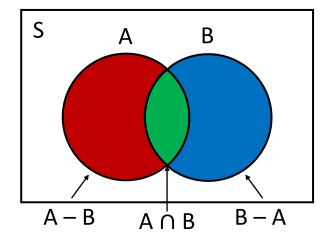
\includegraphics[width=\linewidth]{images/PrincExInVenn.png}
\end{minipage}

\pagebreak

\subsubsection*{Examples}
A computer company receives 350 applications for a job. Suppose that 220 of these applicants majored in computer science, 147 majored in business, and 51 majored in both computer science and business.

\exheader[1] How many of these applicants majored in neither computer science nor business?
\begin{itemize}[leftmargin=*, label={}]
	\item S: set of all applicants $|S| = 350$
	\item C: set of all applicants that majored in CS, $|C| = 220$
	\item B: set of applicants majored in business, $|B| = 147$
	\item Meaning $|C \cap B| = 51$
\end{itemize}
What is $|C' \cap B'|$?
\begin{itemize}[leftmargin=*, label={}]
	\item \sidenote[Its important to remember that all this $|...|$ junk means "size of..."] By DeMorgans law, we know that $|C' \cap B'| = |(C \cup B)'|$
	\item = $|S - (C \cup B)|$ {\tiny by complement definition}
	\item = $|S| - |C \cup B|$ {\tiny from the venn diagram observation}
	\begin{itemize}
		\item Now we just need  $|C \cup B|$, this is where we apply princ of inc/exclusion
	\end{itemize} 
	\item = $|S| - (|C| + |B| - |C \cap B|)$
	\begin{itemize}
		\item Now its just simple substitution
	\end{itemize} 
	\item = 350 - (220 + 147 - 51) = 34.
\end{itemize}

\bigbreak

\exheader[2] How many of these applicants majored in CS but not in business?
\begin{itemize}[leftmargin=*, label={}]
	\item $|C| = 220$ \quad $|B| = 147$ \quad $|C \cap B| = 51$
	\item $|C - B| = |C| - |C \cap B|$ {\tiny from venn diagram}
	\item = 220 - 51 = 169
\end{itemize}

\pagebreak

\subsubsection{Principle of Inclusion and Exclusion (n-way)}

Before looking at the generalized solution, let's look at 3 sets with a venn diagram.
\begin{center}
	\strut\vspace*{-\baselineskip}\newline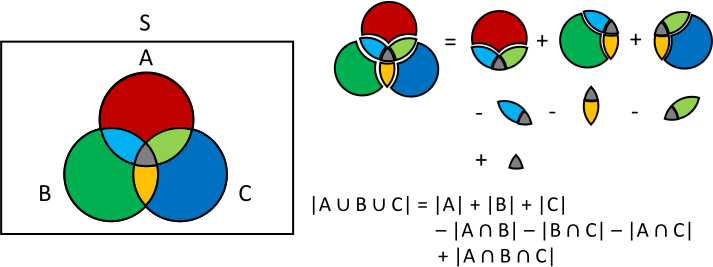
\includegraphics[width=\linewidth]{images/PrinceExInVenn3Way.png}
\end{center}
Notice the pattern? We're first adding the sets then subtracting the intersections every set. Then we add back the intersection of all the sets because just subtracting them would lead to an undercounting issue (we're missing out on the middle piece of the venn diagram).

This pattern can be compiled into our \cul{generalization:} \smallbreak
\begin{tabular}{l l}
	$|A_1 \cup A_2 \cup ... \cup A_n|$ = & $\sum_{1 \le i \le n} |A_i|$ \\
	& $- \sum_{1 \le i < j  \le n} |A_i \cap A_j|$ \\
	& $+ \sum_{1 \le i < j < k \le n} |A_i \cap A_j \cap A_k|$ \\
	& $- \ ...$ \\
	& ... \\
	& $ + (-1)^{n+1} |A_1 \cap A_2 \cap ... \cap A_n|$
\end{tabular} \smallbreak
For example, when $n=3$: \smallbreak
\begin{tabular}{l l}
	$|A_1 \cup A_2 \cup A_3|$ = & $|A_1| + |A_2| + |A_3|$ \\
	& $- |A_1 \cap A_2| - |A_2 \cap A_3| - |A_1 \cap A_3|$ \\
	& $+ |A_1 \cap A_2 \cap A_3|$
\end{tabular}

\pagebreak

\subsubsection*{Examples}
In a class, 19 students are math majors, 23 are CS majors, and 10
are physics majors. In addition, 9 students are math and CS
majors, 2 students are physics and CS majors, 4 students are math
and physics majors. There is 1 student majoring all three majors.

\exheader[1] How many students are there?
\begin{itemize}[leftmargin=*, label={}]
	\item $M$: set of students majoring in math, |M| = 19
	\item $C$: set of students majoring in CS, |C| = 23
	\item $P$: set of students majoring in physics, |P| = 10
	\item $|M \cap C| = 9$, $|P \cap C| =2$, $|M \cap P| = 4$, and $|M \cap C \cap P| = 1$
	\item Answer: $|M| + |C| + |P| - |M \cap C| - |P \cap C| - |M \cap P| + |M \cap C \cap P|$
	\item \quad \quad \quad = 19 + 23 + 10 - 9 - 2 - 4 + 1 = 38.
\end{itemize}
\bigbreak
\exheader[2] How many students major in math only?
\begin{itemize}[leftmargin=*, label={}]
	\item $|M| = 19$, $|C| = 23$, $|P| = 10$
	\item $|M \cap C| = 9$, $|P \cap C| =2$, $|M \cap P| = 4$, and $|M \cap C \cap P| = 1$
	\item Need $|M - (C \cup P)|$ \\
	\begin{tabular}{l l}
		$ = |M| - |M \cap (C \cup P)|$ & (Venn: $|A - B| = |A| - |A \cap B|$) \\
		$ = |M| - |(M \cap C) \cup (M \cap P)|$ & (Distributive Law) \\
		$ = |M| - (|M \cap C| + |M \cap P| - |M \cap C \cap P|)$ & (Principle of I\&E). \\
		$ = 19 - (9 + 4 - 1) = 7$
	\end{tabular}
\end{itemize}
\bigbreak
\exheader[3] How many students major in math or CS but not physics?
\begin{itemize}[leftmargin=*, label={}]
	\item $|M| = 19$, $|C| = 23$, $|P| = 10$
	\item $|M \cap C| = 9$, $|P \cap C| =2$, $|M \cap P| = 4$, and $|M \cap C \cap P| = 1$
	\item Need $|M \cup C - P|$ \\
	\begin{tabular}{l l}
		$ = |M \cup C| - |(M \cup C) \cap P|$ & (Venn: $|A - B| = |A| - |A \cap B|$) \\
		$ = |M \cup C| - |(M \cap P) \cup (C \cap P)|$ &  (Distributive) \\
		$ = |M| + |C| - |M \cap C| - (|M \cap P| + |C \cap P| - |M \cap C \cap P|)$ &  \\
		$ = 19 + 23 - 9 - (4 + 2 - 1) = 28$
	\end{tabular}
\end{itemize}

\pagebreak


\subsubsection{Pigeonhole Principle}
\define[If more than k pigeons are placed into k pigeonholes, then at least one hole contains more than one pigeon. This principle is used to answer questions of the form "at least how many objects satisfy a certain property"]
\vspace*{-0.3cm} \\ To use the pigeonhole principle, we need to;
\begin{itemize}[label={\faAngleRight}]
	\item Identify "pigeons" and identify "pigeonholes"
	\item Associate between pigeons and pigeonholes.
\end{itemize}

\bigbreak

\cul{Generalization:} If n objects are placed into k boxes, then there is at least one box containing at least \sidenote[The "ceiling" operation rounds up to the nearest whole integer. ex; $\ceil{2.2} = 3$] $\underbrace{\ceil{n/k}}_\textrm{"ceiling" of}$ objects.
\smallbreak This can be proven by contradiction;
\begin{itemize}[label={\faAngleRight}]
	\item Assume to the contrary that none of the boxes contain more than $\ceil{n/k} - 1$ objects.
	\item Then the total number of objects is at most; $k(\ceil{n/k} -1 ) < k((n/k + 1) - 1) =n$
	\item This is a contradiction because there are a total of $n$ objects.
\end{itemize}



\bigbreak

\subsubsection*{Examples}

\begin{minipage}[t]{0.75\linewidth}
\exheader[1] Seven points lie inside a hexagon of side length 1. \\ Show that there must exist at least two points whose distance apart is at most 1.
	\begin{itemize}[leftmargin=*, label={}]
		\item Pigeons: points.
		\item Pigeonholes: Triangles
		\begin{itemize}
			\item We can set up our pigeonhole by dividing our hexagon into 6 triangles. The lengths of these triangle sides are at most one, so the distance between any two points contained in the triangle can be at most one.
		\end{itemize} 
		\item At least two points are inside one of these triangles by pigeonhole principle, so at least one set of points satisfies the "distance of at most one" setup from the triangle info above.
	\end{itemize}
\end{minipage}
\begin{minipage}[t]{0.15\linewidth}
    \begin{center}
		\strut\vspace*{-\baselineskip}\newline\hspace*{0.5cm}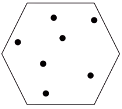
\includegraphics[width=\linewidth]{images/pigeon/hex.png}
		\strut\vspace*{-\baselineskip}\newline\hspace*{0.5cm}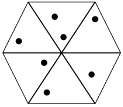
\includegraphics[width=\linewidth]{images/pigeon/hex2.png}	
	\end{center}
    
\end{minipage}

\pagebreak

\exheader[2] There are some people in a room. Some are acquaintances; some are not. Assume that if a is acquainted to b, then b is acquainted to a. Also, no one is acquainted to him- or herself.  Show that at least two people have the same number of acquaintances.
\begin{itemize}[leftmargin=*, label={}]
	\item Let n be the number of people in the room.
	\item Pigeons: People in the room.
	\item Pigeonholes: Number of acquaintances.
	\begin{itemize}
		\item Possible acquaintances: $0,1,2 ... , n-1$
	\end{itemize}
\end{itemize}
Two Possible Cases:
\begin{enumerate}
	\item Someone has 0 acquaintances
	\begin{itemize}[label={\faAngleRight}]
		\item {\small This implies that no one has $n-1$ acquaintances.}
		\item {\small Pigeonholes = $\{0,1,2,...,n-2\}, n-1$ pigeonholes. $n$ pigeons.}
	\end{itemize}
	\item No one has 0 acquaintances
	\begin{itemize}[label={\faAngleRight}]
		\item {\small Pigeonholes = $\{1,2,...,n-1\}, n-1$ pigeonholes. $n$ pigeons.}
	\end{itemize}
\end{enumerate}
By pigeonhole principle, there must be 2 people that have the same number of acquaintances. 

\bigbreak

\exheader[3] Among 15 students, at least how many were born on the same day of the week?
\begin{itemize}[leftmargin=*, label={}]
	\item Objects: students 
	\item Boxes: days of the week 
	\item There are at least $\ceil{15/7} = 3$ students born on the same day of the week.
\end{itemize}

\bigbreak

\exheader[4] How many students, each of whom comes from one of the 50 states, must be enrolled in a university to guaranteed that there are at least 100 who come from the same state?
\begin{itemize}[leftmargin=*, label={}]
	\item Objects: students.
	\item Boxes: 50 states.
\end{itemize}
However, this time we don't know the number of students.
\begin{itemize}[label={\faAngleRight}]
	\item We want to find the minimum n so that $\ceil{n/50} = 100$
	\item This happens when the quotient is 99 and the remainder is 1.
	\item Thus, $ n = 50 * 99 + 1 = 4951$
\end{itemize}

\pagebreak

\subsection{Permutation and Combination}
\begin{minipage}[t]{0.9\linewidth}
	Many counting problems can be solved by finding the number of ways to select a specified number of objects out of a set. \smallbreak
	When order matters: Permutations. \\
	When order doesn't matter: Combinations. \smallbreak
	For example: 
	\begin{itemize}[leftmargin=*, label={}]
		\item In how many ways  can we select three students from a group of students to stand in line for a picture?
		\begin{itemize}
			\item Order matters here, so permutation
		\end{itemize}
		\item How many different committees of three students can be formed from a group of five students?
		\begin{itemize}
			\item Order doesn't matter here, so combinations
		\end{itemize}
	\end{itemize}
\end{minipage}
\fbox{\tiny
	\begin{minipage}[t]{0.22\textwidth}
		Recall: 
		\begin{itemize}[leftmargin=*, label={}]
			\item Multiplication Principle
			\begin{itemize}[leftmargin=0.2cm, label={}]
				\item $|A \times B| = |A| \cdot |B|$
			\end{itemize}
			\item 
			\item Addition Principle
			\begin{itemize}[leftmargin=0.2cm, label={}]
				\item $| A \cup B| = |A| + |B|$
			\end{itemize}
			\item  
			\item Prnc' of Inclsn \& Exclsn
			\begin{itemize}[leftmargin=0.1cm, label={}]
				\item $| A \cup B | = |A| + |B| - |A \cap B|$
			\end{itemize}
		\end{itemize}
	\end{minipage}
}


\end{document} 




 